\documentclass[12pt]{article}
\input{settings}

% for specifying font sizes of section headings
\usepackage{sectsty}
\sectionfont{\fontsize{14}{15}\selectfont}

% bib options
\let\oldbibliography\thebibliography
\renewcommand{\thebibliography}[1]{\oldbibliography{#1}
\setlength{\itemsep}{0pt}} 
\usepackage[numbers,sort&compress]{natbib} 
\bibliographystyle{unsrtnat}

% for writing some symbols
\usepackage{gensymb}
\usepackage{textcomp}

% landscape pages
\usepackage{lscape}

% long tables to go with landscape mode
\usepackage{longtable}

% for spaces between paragraphs
\usepackage[parfill]{parskip}

% for tables
\usepackage{booktabs}
\renewcommand{\arraystretch}{1.5}

% for wrapping text around figures
\usepackage{wrapfig}

% margins and lines
\usepackage[margin=2.5cm]{geometry}
\pagestyle{fancy} 
\fancyheadoffset[R]{0.2cm}
\usepackage{lineno} 

% editing and track changes
\newcommand{\emck}[1]{\textcolor{blue}{$^{\textrm{emck}}${#1}}}
\newcommand{\edit}[1]{\textcolor{red}{#1}}

% title and authors
\title{\vspace{-1.8cm}\Large{\textbf{Investigando la biofísica de la
      respiración usando electromiografía y espirometría}}} \author{}
%\author[1, \email]{Erin C. McKiernan} 

%\affil[1]{\small{Departamento de F\'isica, Facultad de Ciencias, Universidad Nacional Aut\'onoma de M\'exico}}

%\affil[ \email]{\small{emckiernan@ciencias.unam.mx}}
\date{}

%%%%%%%%%%%%%%%%%%%%%%%%%%%%%%%%%%%%%%%%%%%%%%%%%%%%%%%%%%%%
 
\begin{document}
\maketitle

\vspace{-1.4cm}

\section*{RESUMEN}

En este práctica de laboratorio, los estudiantes usarán un espirómetro
para registrar el volumen de aire inhalado y exhalado durante
respiración normal y forzada mientras simultáneamente
registran electromiogramas de diferentes músculos respiratorios. En
general, esta práctica ayudará a los estudiantes entender la mecánica
de la respiración y comprender la relación entre la activación
eléctrica de los músculos respiratorios y el volumen de aire inhalado
o exhalado.

\section*{ESPECIFICACIONES}
\begin{tabular}{p{6cm} p{10cm}}
\textbf{Nivel de estudio:} & Licenciatura \\
\textbf{Carreras:} & Biología, Física, Física Biomédica, otros \\
\textbf{Semestere:} & 4to a 6to (i.e. alumnos de 2do o 3ro año) \\ 
\textbf{Para uso en materias:} & Fisiología de Sistemas, Física del Cuerpo Humano, otros \\
\textbf{Prerequisitos recomendados:} & Biología Molecular \& Celular \\
\textbf{Duration of practical:} & 2 horas \\
\textbf{Setting:} & Aula o laboratorio \\
\textbf{Precauciones:} & Tenga sillas disponibles para que los participantes se sienten en caso de que respiración repetida y forzada provoca mareo; Use filtros boquillas desechables y desinfecte el espirómetro entre sujetos para evitar la transmisión de los gérmenes. \\
\textbf{Otras indicaciones:} & Usar ropa comoda para permitar respiración sin impedimentos y colocación de los electrodos
\end{tabular}

\section*{OBJETIVOS}
\textbf{Antes de hacer esta práctica el estudiante debe ser capaz de:}
\begin{itemize}
\item describir la anatomía de los pulmones y el sistema respiratorio
\item identificar y ubicar los músculos respiratorios primarios y accesorios
\item explica como los músculos contren y se relajan
\end{itemize}
 
\vspace{0.3cm}

\emck{Througout this practical and others, I have doubts about the best way to translate 'you'. formal/informal? plural/singular?}

\textbf{En este práctica \emck{podrá/hará}:}
\begin{itemize}
\item aprender como usar un espirómetro
\item aprender como registrar electromiogramas (EMGs)
\item observar y registrar los cambios en el volumen de aire cuando
  inhalas y exhalas
\item observar y registrar la activación de diferentes grupos de
  músculos durante la inhalación y la exhalación
\item investigar cómo los volúmenes y las activaciones musculares difieren entre la respiración normal y la forzada
\end{itemize}

\vspace{0.3cm}
 
\textbf{Después de la práctica debe ser capaz de:}
\begin{itemize}
\item entender la mecánica básica de la respiración
\item describir el papel de los músculos primarios versus accesorios en la respiración
\item explicar como la respiración normal y forzada difieren
\item explicar la relación entre contracción de músculos diferentes y cambios en volumen
\item diseñar experimentos adicionales para investigar como la respiración cambia bajo condiciones diferentes
\end{itemize}

\section*{EQUIPO}

\textbf{Para espirometría:}
 \begin{itemize}
	\item Espirometro (e.g. modelo Vernier SPR-BTA)
   	\item Filtros bacterianos desechables (Vernier)	
	\item Boquillas desechables (Vernier)
        \item Clip de nariz (Vernier)
	\item LabQuest 2 \emck{standalone interface?}  (Vernier)
        \item Computadora con el software de Logger Pro (Vernier) instalado para analizar datos (opcional), o
        \item Computadora con Python instalado para analizar datos (opcional)
        \item Solución de limpieza (i.e. Spray o toallitas de Lysol)
\end{itemize}

\vspace{0.3cm}

\textbf{Para electromiografía:}
 \begin{itemize}
	\item Muscle SpikerBox (Backyard Brains)
        \item 3 electrodos de superficie (Backyard Brains o otro proveedor)
        \item cable naranja con pinzas de cocodrilo para conectar los electrodos al SpikerBox (Backyard
Brains)
    \item cable para conectar el SpikerBox a una computadora, tableta, o télefono inteligente (Backyard
Brains)
 	\item tableta, computadora o teléfono inteligente con el software gratuito Backyard Brains Spike
Recorder instalado
\end{itemize}


\section*{ANTECEDENTES}

\subsection*{Tipos de respiración}

La respiración se puede dividir en dos tipos según el esfuerzo
ejercido y los músculos involucrados: (1) respiración normal (eufnea),
que se lleva a cabo en condiciones de reposo, y (2) respiración
forzada (hiperpnea), que ocurre cuando la demanda de oxígeno del el
cuerpo aumenta, por ejemplo, durante el ejercicio
\cite{openStax2016resp}. La inhalación normal es un proceso activo
durante lo cual los músculos inspiratorios primarios (ver a continuación) se
activan. La exhalación normal es un proceso pasivo durante lo cual los
pulmones regresan a su posición de reposo debido al retroceso (\emck{recoil})
elástico. La inhalación forzada involucra esfuerzo adicional para
traer más que el volumen de aire normal a los pulmones, y requiere la
activación de grupos de músculos adicionales. La exhalación forzada, a
diferencia de la exhalación normal, es un proceso activo que requiere
la activación de músculos selectos para comprimir la cavidad torácica
 y los pulmones más allá del punto de retroceso elástico normal y
empujar el aire adicional fuera de los pulmones \cite{openStax2016resp}.

\subsection*{Músculos respiratorios y la mecánica de la respiración}

Los músculos involucrados en la respiración pueden ser clasificados
como primarios o accesorios dependiendo de si están activados durante
la respiración normal o forzada, respectivamente
\cite{sieck2013mechanical}.

\subsubsection*{Músculos respiratorios primarios}

Los músculos primarios inspiratorios son el diafragma y los
intercostales externos (Fig. \ref{fig:primary})
\cite{openStax2016resp}. El diafragma se contrae, moviéndose hacia
abajo para aumentar el volumen de la cavidad torácica en el eje
vertical \cite{guyton20006textbook}.

Los intercostales externos contraen, jalando de la caja torácica hacia
arriba y hacia afuera para expandir la cavidad torácica en el eje
anterior a posterior. Durante la exhalación, el diafragma y los
intercostales externos simplemente se relajan, volviendo a sus
posiciones de reposo debido a las propiedades de retroceso elástico de
los pulmones y disminuyendo el volumen de la cavidad torácica
\cite{guyton20006textbook}. Por lo tanto, la inhalación normal es un
activo proceso que requiere la activación del diafragma y externo
intercostales, mientras que la exhalación normal es un proceso pasivo
que implica relajación muscular y retroceso elástico de los pulmones
\cite{guyton20006textbook}. Por lo tanto, la inhalación normal es un
proceso activo que requiere la activación del diafragma y los
intercostales externos, mientras que la exhalación normal es un
proceso pasivo que implica relajación muscular y retroceso elástico de
los pulmones \cite{openStax2016resp}.

\begin{figure}[h!]
\centering
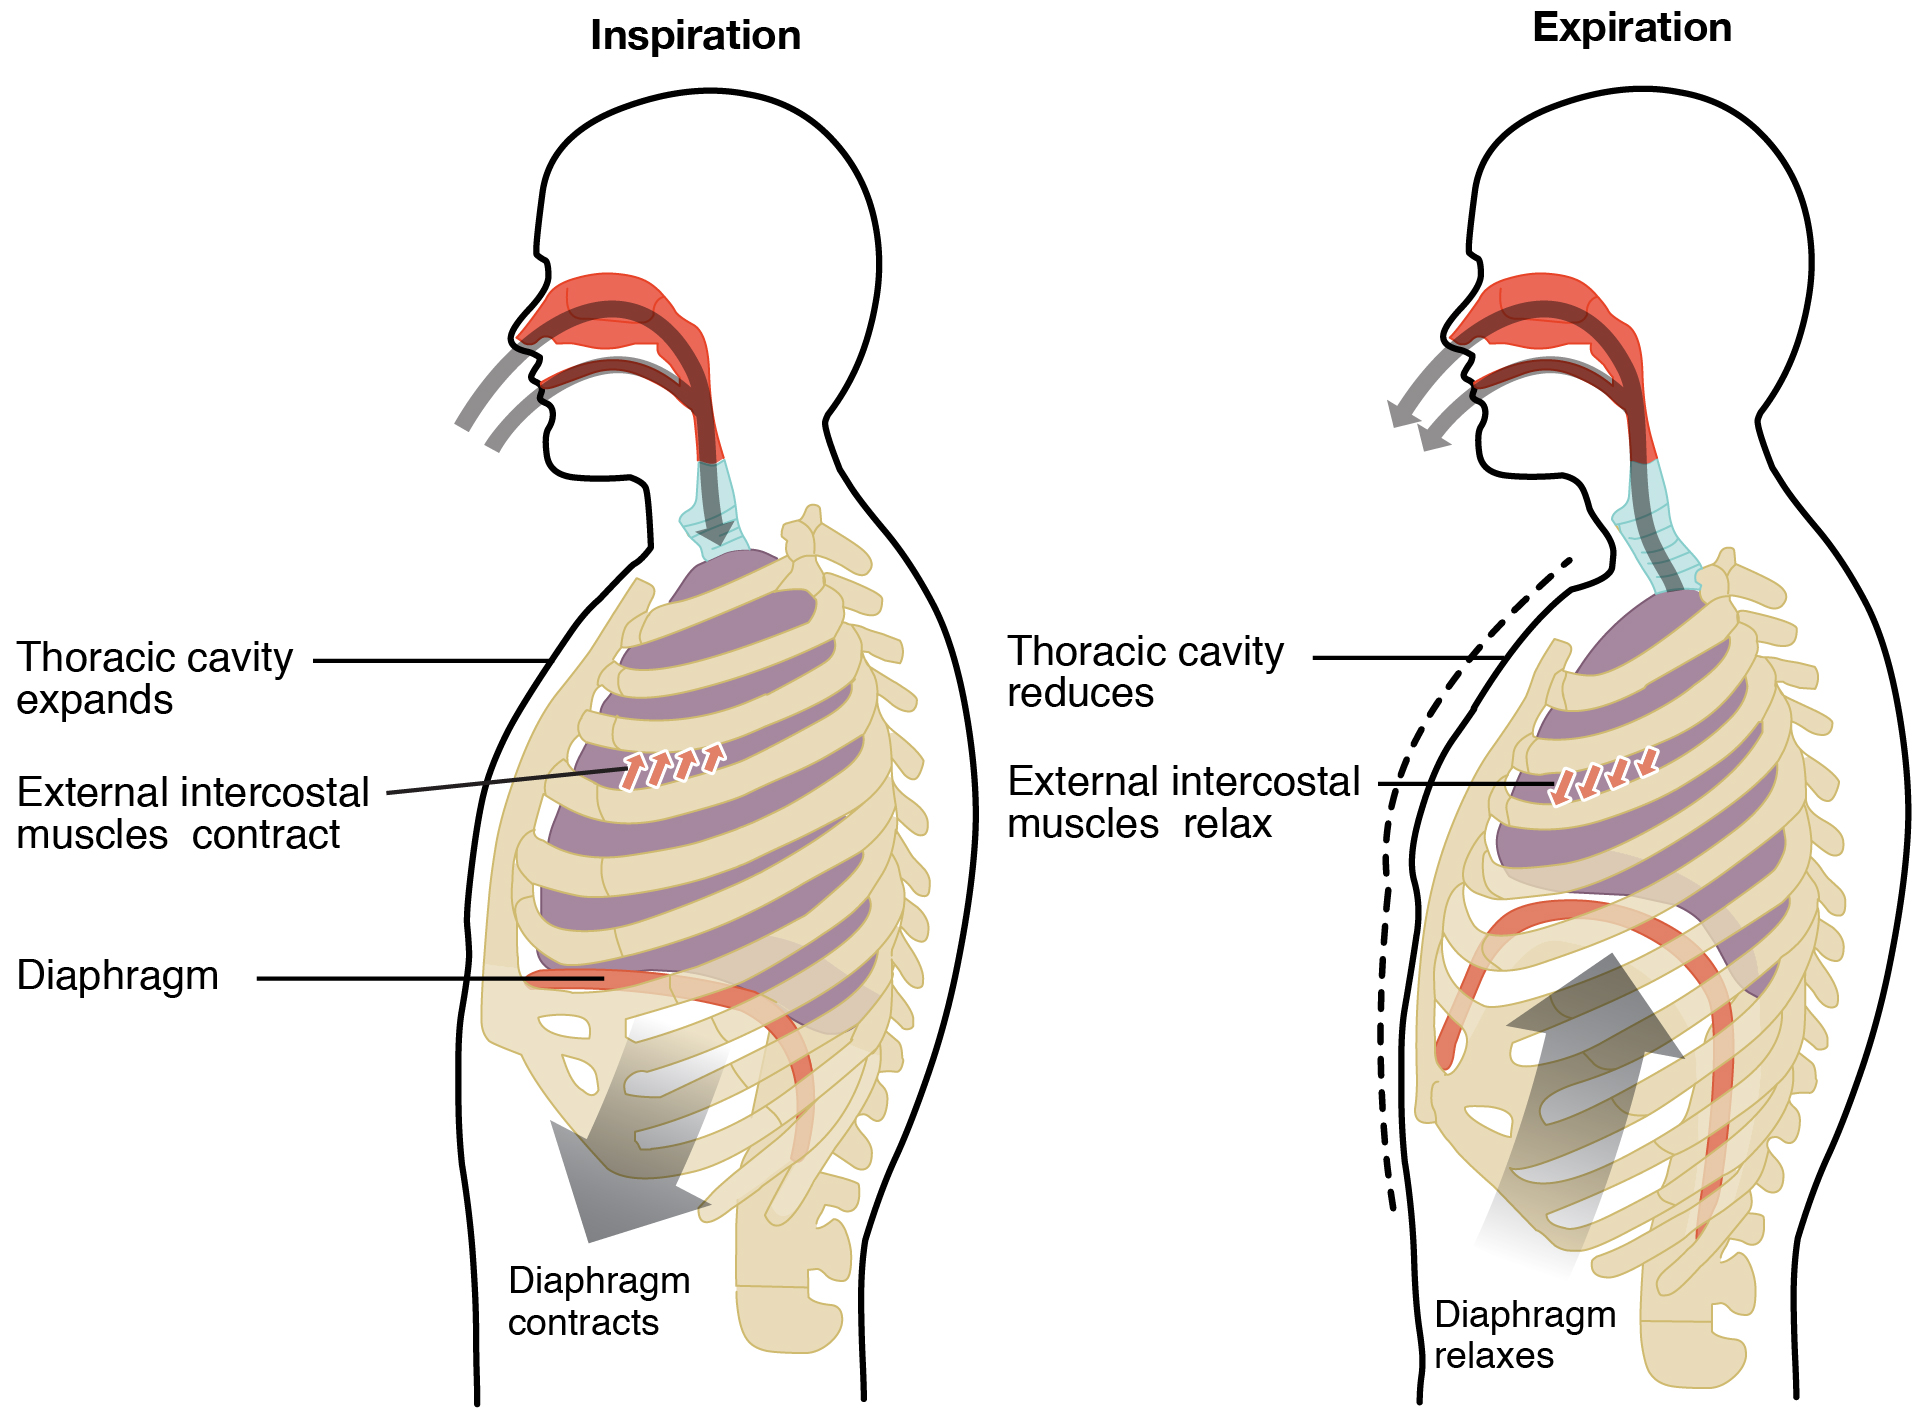
\includegraphics[width=0.7\textwidth]{images/Inspiration_and_Expiration.jpg}
\caption{Movimiento del diafragma y los músculos intercostales
  externos durante la inspiración y expiración. Crédito del imagen:
  OpenStax CNX \cite{openStax2016resp}, Creative Commons Attribution
  license (CC BY).}
\label{fig:primary}
\end{figure}

\subsubsection*{Músculos respiratorios accesorios}

Los músculos accesorios son aquellos que solo se activan durante
respiración forzada, cuando se requiere un esfuerzo adicional para
extraer más aire \emck{pull more air in} o empujar más aire hacía
fuera de los pulmones \cite{openStax2016resp,sieck2013mechanical}. Los
músculos accesorios involucrados en la inhalación forazada se muestran
en Fig. \ref{fig:acc_insp} e incluyen el esternocleidomastoideo, el
escalenos, el serrato anterior y el pectoral menor, entre otros
\cite{troyer1986action,ratnovsky2008mechanics}. Estos músculos,
encontrados en los áreas del cuello y el pecho, actúan para expandir
el volumen del cavidad torácica más allá de lo que se puede lograr
solo con los músculos inspiratorios primarios y traen más aire. Los
músculos accesorios involucrados en la expiración forzada se muestra
en la Fig. \ref{fig:acc_exp} e incluyen los intercostales internos,
traversus thoracis, oblicuo externo, oblicuo interno y recto abdominis
\cite{troyer1986action,ratnovsky2008mechanics}. Estos músculos,
ubicados en el pecho y las áreas abdominales, actúan para reducir aún
más el volumen de la cavidad torácica y expulsar más aire de los
pulmones de lo que puede se lograr mediante el simple retroceso
elástico.

\begin{figure}[h!]
\centering
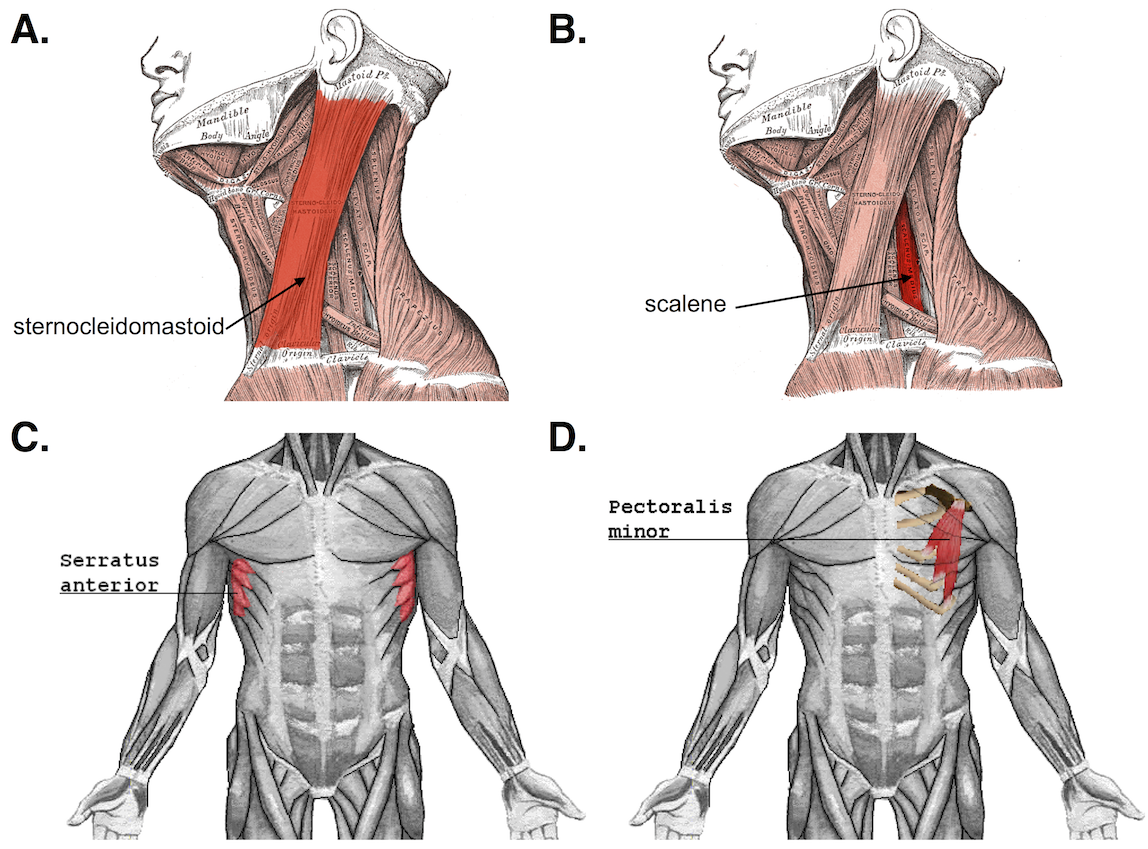
\includegraphics[width=0.75\textwidth]{images/accessory_insp.png}
\caption{Músculos inspiratorios accesorios. Créditos de los imágenes::
  A.,B. imágenes \emck{highlighted} de Gray's Anatomy (1858), dominio
  público; C.,D. Originales por sv:Anv\"andare:Chrizz via Wikimedia
  Commons, Creative Commons Attribution-ShareAlike license (CC
  BY-SA).}
\label{fig:acc_insp}
\end{figure}%

\begin{figure}[h!]
\centering
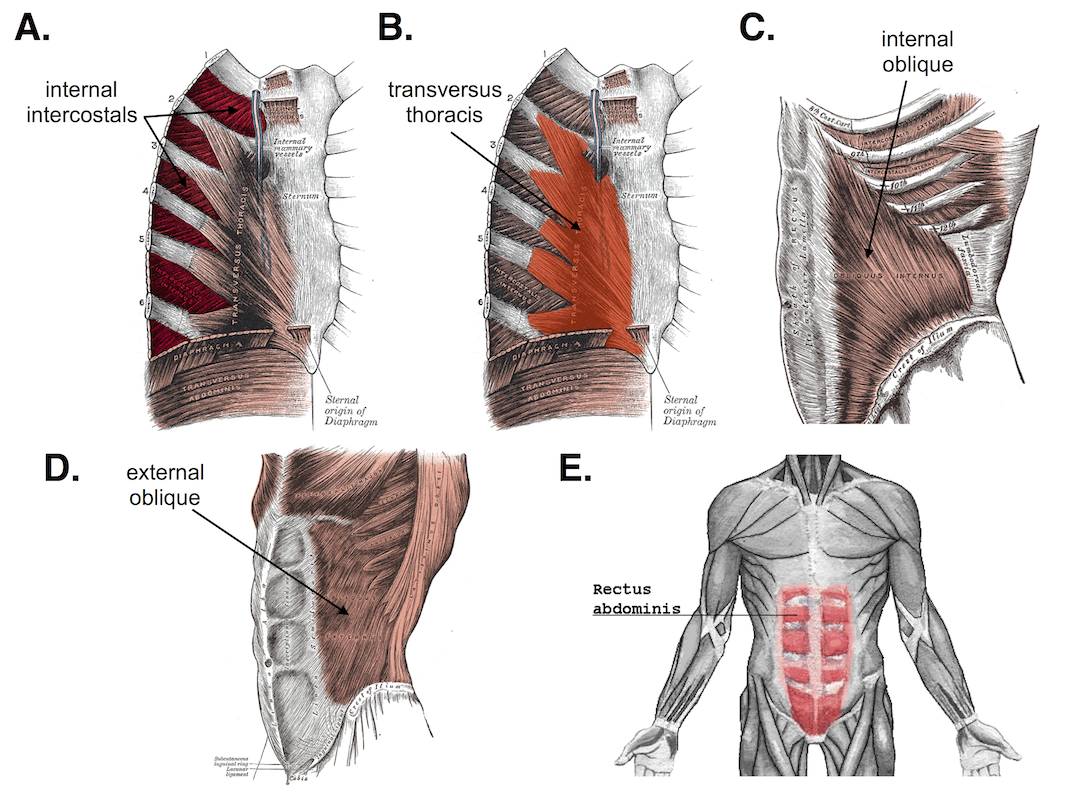
\includegraphics[width=0.76\textwidth]{images/accessory_exp.png}
\caption{Músculos expiratorios accesorios. Créditos de los imágenes:
  A-D. imágenes \emck{highlighted} de Gray's Anatomy (1858), dominio
  público; E. Original por sv:Anv\"andare:Chrizz via Wikimedia Commons,
  CC BY-SA.}
\label{fig:acc_exp}
\end{figure}

\subsection*{Medición de la actividad de los músculos respiratorios - electromiograma}

Los músculos están compuestos de células excitables que generan
impulsos eléctricos, llamados potenciales de acción (APs). El disparo
de APs \emck{AP firing} inicia cascadas de eventos de señalización
celular que finalmente conducen \emck{lead to?} a la contracción
muscular. (Para una revisión de la fisiología muscular y acoplamiento
de excitación-contracción, ver Cap. 6-7 en \cite{guyton20006textbook}
y también \cite{sieck2013mechanical}.) Por lo tanto, la actividad
eléctrica en los músculos está acoplado a la actividad contráctil.

Para registrar la actividad eléctrica de los músculos usamos una
técnica llamada electromiografía, y los registros que obtenemos se
llaman electromiogramas (EMGs) \cite{garcia2011surface}. El registro
de EMG puede ser hecho de forma invasiva mediante la
inserción de electrodos en el músculo de interés, o de forma no
invasiva mediante el uso de electrodos de superficie colocados en la
piel encime del músculo (Fig. \ref{fig:emg}).

La inserción de electrodos tiene la ventaja de dar registros EMG ``más
limpias'' en las cuales la actividad de las unidades motoras
\emck{separadas/individuales?} se pueden distinguir. Sin embargo, la
inserción de electrodos puede ser doloroso y requiere condiciones
estériles para prevenir la infección, lo que hace este tipo de
registro no ideal para la configuración del aula \emck{classroom
  setting?}. Electrodos de superficie, por el contrario, pueden
aplicarse y quitarse fácilmente del piel sin lesiones. Las
limitaciones de este tipo de registro extracelular incluye solo poder
grabar desde músculos superficiales, y registros que a menudo
\emck{often} no permiten la separación de las unidades motoras
individuales \cite{garcia2011surface}. Estas limitaciones no son
prohibitivas y tipicamente son superadas por los beneficios de la no
invasividad, pero deben tenerse en cuenta cuando pensando en la
colocación de electrodos y el análisis de datos.

Una de las configuraciones de registro más comunes se conoce como EMG
bipolar, o \emck{single differential EMG}
\cite{garcia2011surface}. Dos electrodos de superficie se colocan en
la piel sobre el músculo solo algunos centímetros aparte
(Fig. \ref{fig:emg}). Al restar las señales registradas en los dos
puntos y luego amplificar la diferencia, señales comunes que pueden
resultar de los músculos fuera del sitio de registro están
\emck{largely} excluidos, y se registra principalmente cambios locales
en actividad. Por lo tanto, esta configuración disminuye la
interferencia muscular \cite{garcia2011surface}.

\begin{figure}[h!]
\centering
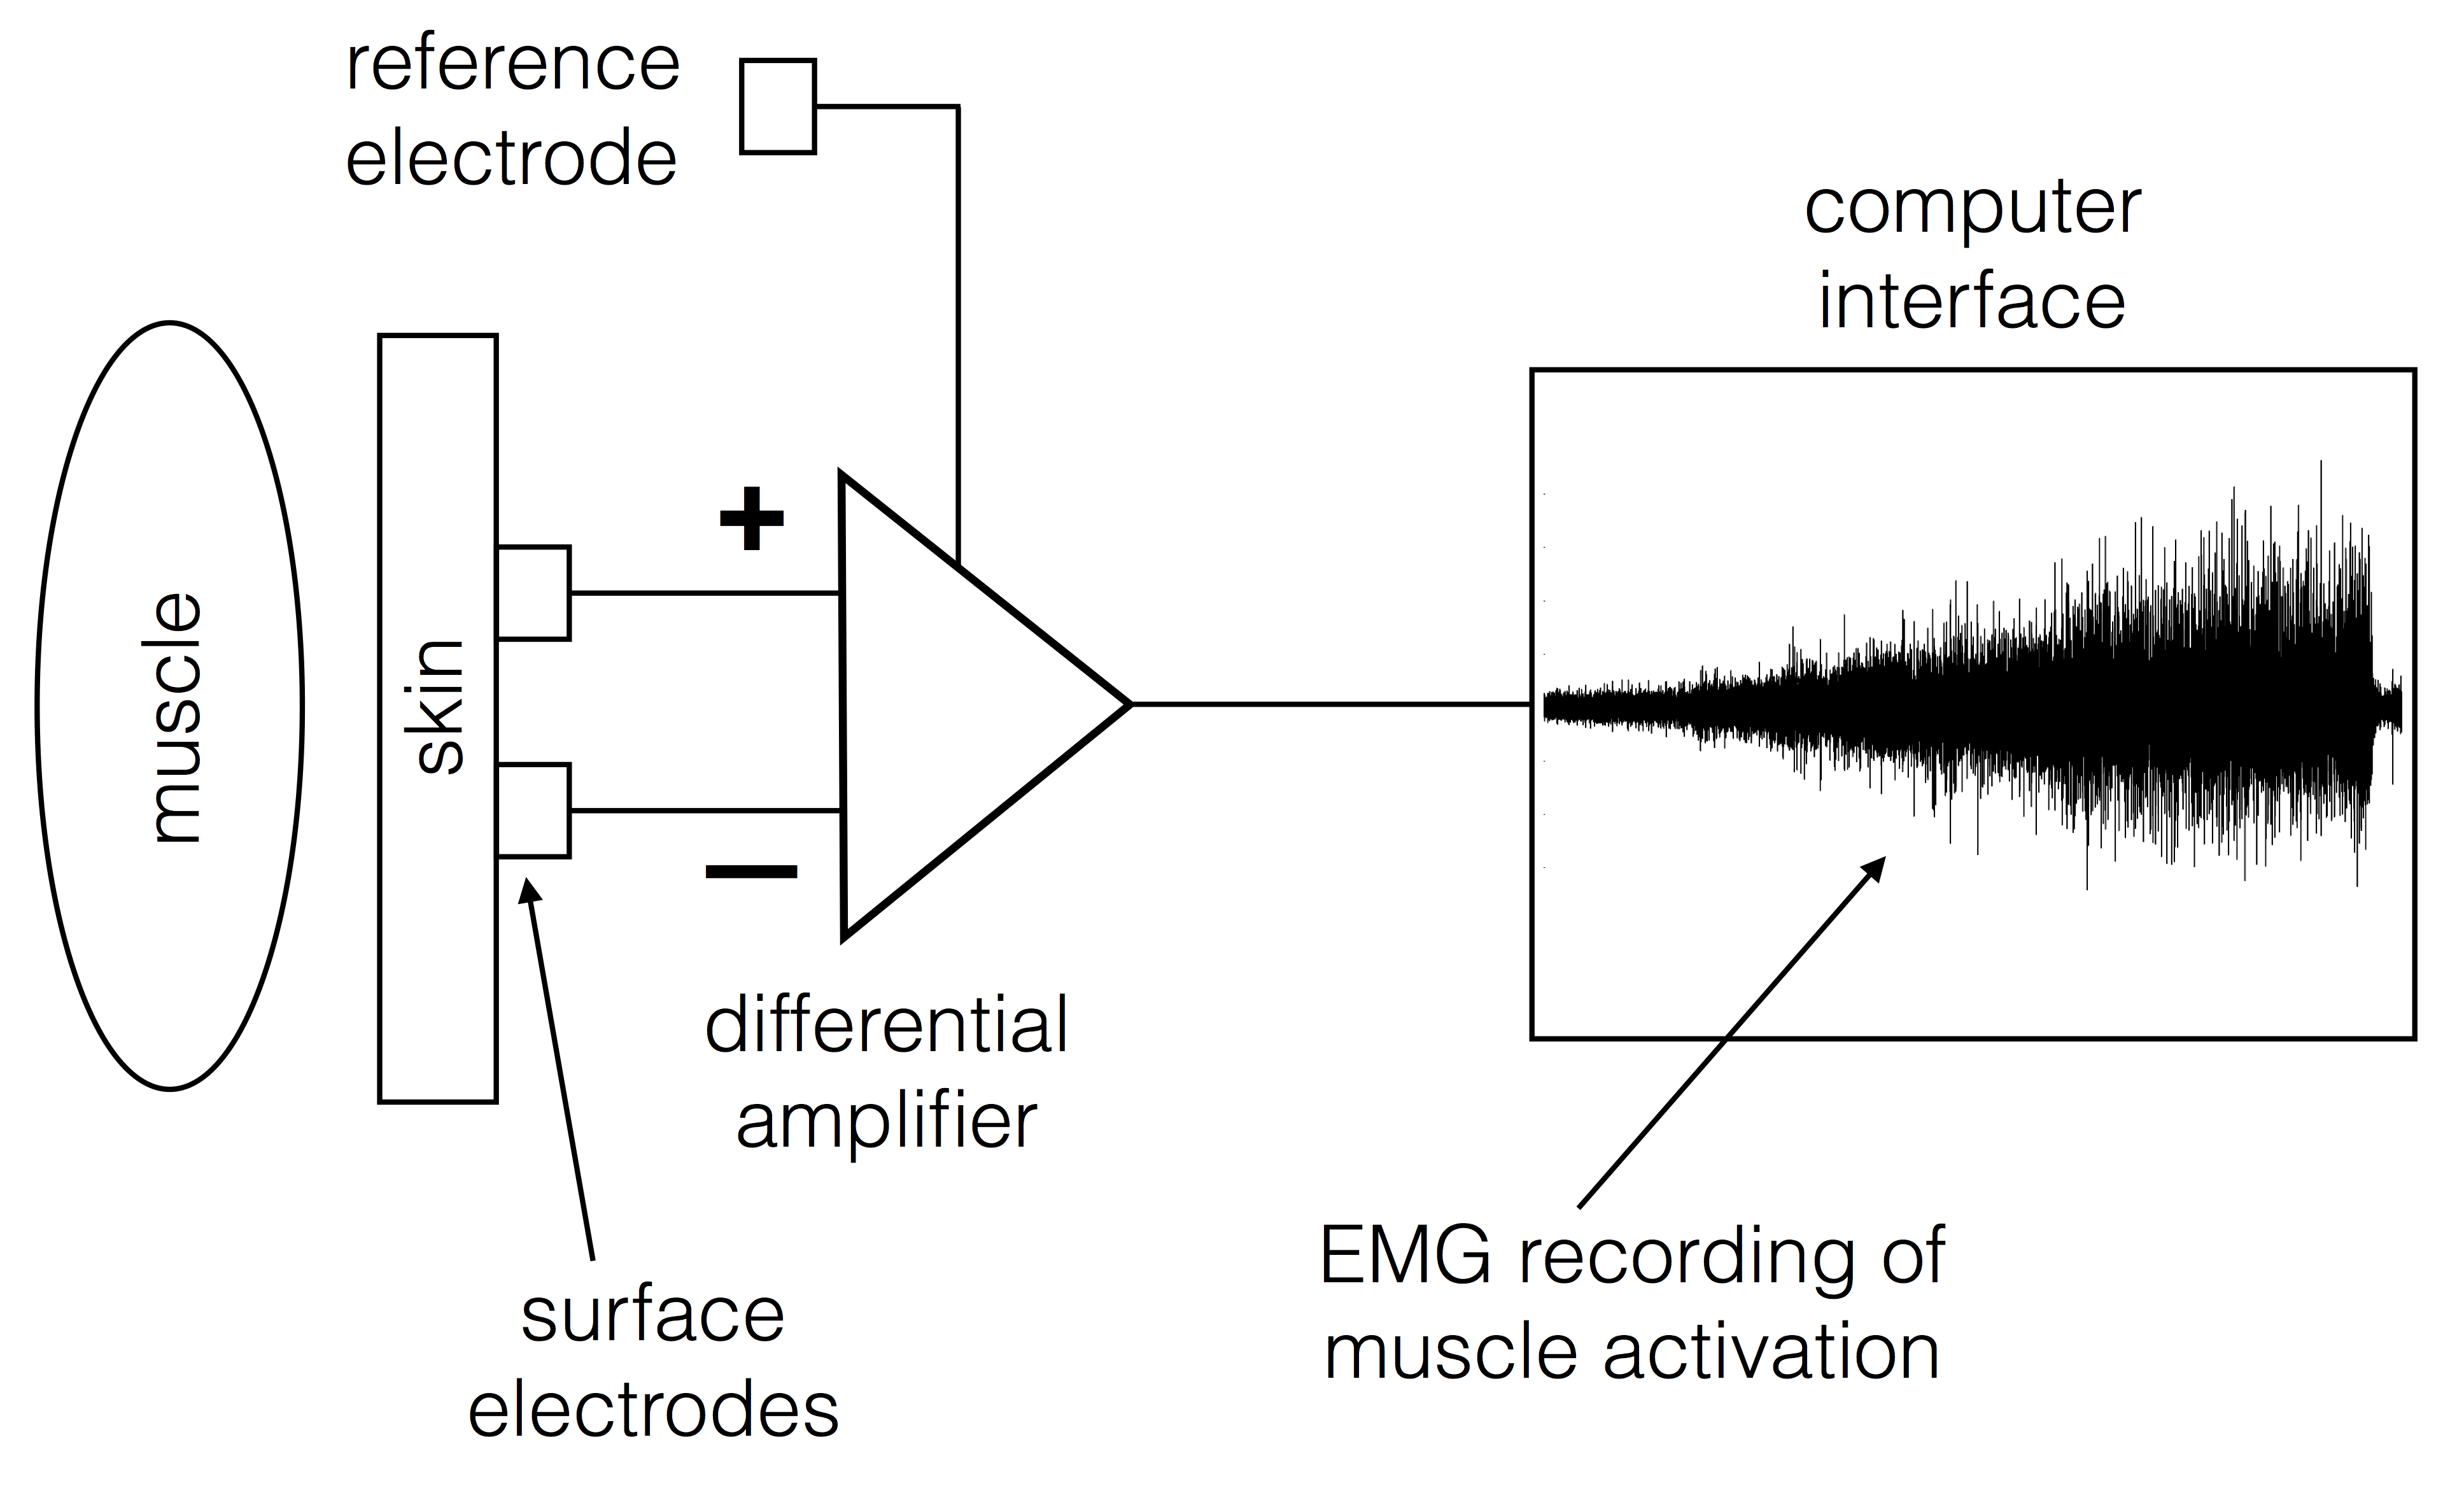
\includegraphics[width=0.7\textwidth]{images/emgAmp.png}
\caption{Configuración del registro EMG bipolar. Para simplificar, no
  todo los componentes del cuerpo o registro se muestren. Crédito de
  imágen: Erin C. McKiernan, CC BY}
\label{fig:emg}
\end{figure}

\emck{Bipolar surface EMGs} pueden decirnos varias cosas sobre la
actividad muscular \cite{garcia2011surface}.

Uno es el \emck{timing?} curso temporal de activación y relajación
muscular. La mayoría de los músculos muestran muy poco actividad en
reposo. Cuando se activa, vemos un aumento notable en la ocurrencia de
impulsos eléctricos, como se muestra en la Fig. \ref{fig:emg} (lado
derecho). Cuando el músculo se relaja, estos impulsos desaparecen y
registramos solo el ruido de referencia \emck{baseline?}. El curso
temporal de la actividad muscular luego se puede correlacionar con
otras medidas; por ejemplo, en el caso de esta práctica, con el
volumen de aire inhalado y exhalado. Podemos también, hasta cierto
punto, estimar la fuerza o el esfuerzo ejercido durante una
contracción. A medida \emck{mientras?} que el sujeto aumenta la fuerza
de contracción, vemos un aumento en la frecuencia de los impulsos
eléctricos y la amplitud de la señal. Estos cambios son el resultado
de dos factores: (1) una mayor frecuencia de disparo en unidades
motoras ya activas, y (2) el reclutamiento de unidades motoras
adicionales. Recuerde, estamos registrando la actividad de unidades
motoras múltiples. Con el aumento de la fuerza de contracción, se
reclutan más unidades motoras y comienzan a disparar, su actividad se
suma, y contribuyen al aumento en la frecuencia y amplitud.


\subsection*{Preguntas de estudio} 
\begin{enumerate}
\item ¿Dónde tendrá que colocar los electrodos para registrar los EMGs
  de los músculos inspiratorios primarios? Dibuja la ubicación de
  los músculos y la colocación de electrodos.
\item ¿Dónde tendrá que colocar los electrodos para registrar los EMGs
  de los músculos inspiratorios o expiratorios accesorios? Dibuja la
  ubicación de los músculos y la colocación de electrodos.
\item ¿Podrás grabar de todos los grupos de músculos? ¿Por qué o por qué no?
\item ¿Cuáles músculos probablemente te darán los mejores registros
  para cada tipo de respiración? ¿Por qué?
\item ¿Cómo sabrá si ha colocado correctamente los electrodos?
\end{enumerate}

\subsection*{Relaciones presión-volumen durante la respiración}
La activación y relajación de los músculos respiratorios causa el
volumen de los pulmones de aumentar o disminuir, como se describió
anteriormente. Estos cambios de volumen, a su vez, causan cambios de
presión de acuerdo con la Ley de Boyle, que dice \emck{states} que la
presión de un gas es inversamente proporcional a su volumen en un
sistema cerrado. En otras palabras, como el volumen aumenta, la
presión disminuye, y viceversa (Fig. \ref{fig:boyle}).

\begin{figure}[h!]
\centering
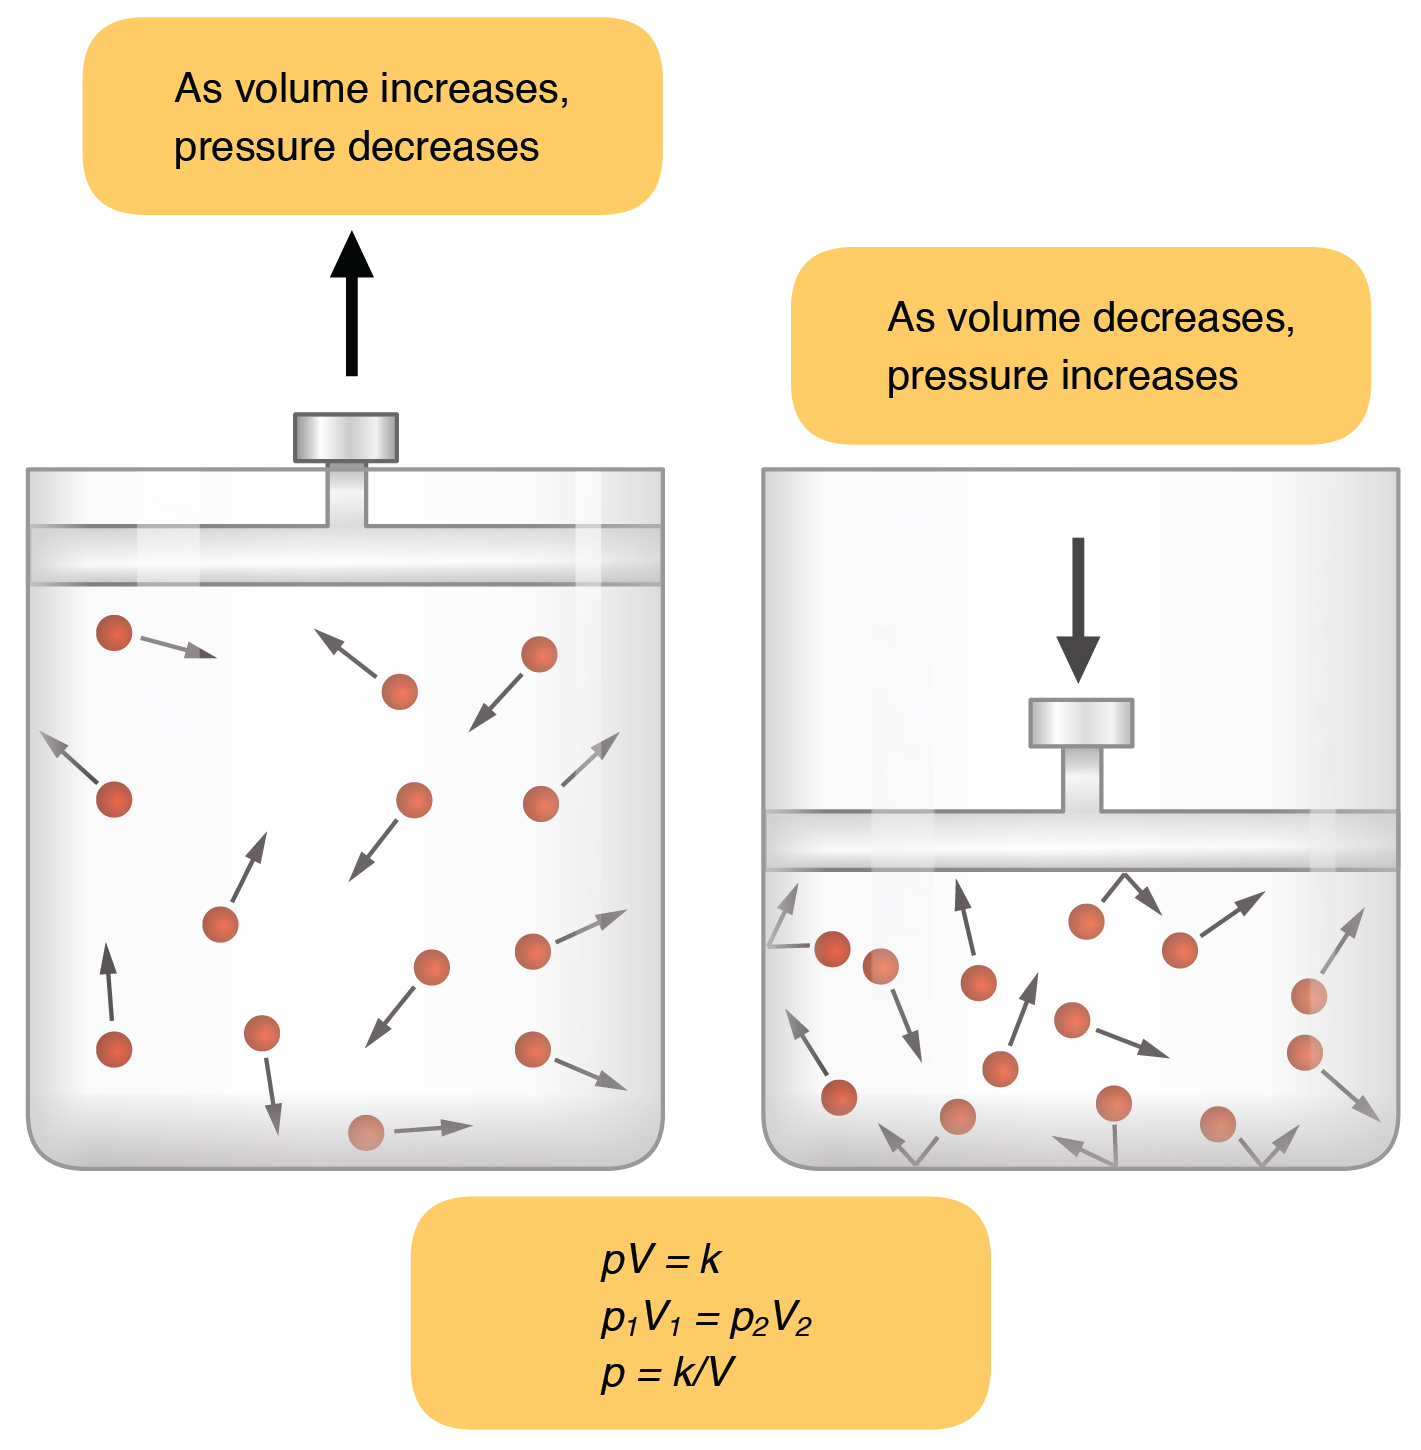
\includegraphics[width=0.6\textwidth]{images/Boyles_Law.jpg}
\caption{Representación esquemática de la Ley de Boyle, donde p es
  presión, v es el volumen y k es un constante. Crédito de imagen:
  OpenStax CNX \cite{openStax2016resp}, CC BY.}
\label{fig:boyle}
\end{figure}

De forma análoga a la Ley de Ohm para flujo de corriente, el flujo de
aire es proporcional al gradiente de presión
\cite{sanchez2010respiratory}:

\begin{equation}
Q= \frac{P_1 - P_2}{R}
\label{eq:ohmFlow}
\end{equation},

donde $\dot{Q}$ es la velocidad del flujo, $P_1$ y $P_2$ son los
presiones en los puntos inicial y final de una vía, y $R$ es la
resistencia del camino. En el sistema respiratorio, las presiones de
interés son las presiones atmosférica ($P_{atm}$) and la alveolar
($P_{alv}$), y la resistencia es la de las vías respiratorias
($R_{aw}$) \cite{sanchez2010respiratory}. Por lo tanto, podemos
reescribir la Ecuación \ref{eq:ohmFlow} como,

\begin{equation}
Q= \frac{P_{atm} - P_{alv}}{R_{aw}}.
\label{eq:ohmFlowResp}
\end{equation},

El aire fluye por un gradiente de presión desde un área de mayor a
menor presión. Por lo tanto, durante la inspiración, el diafragma y
los intercostales externos actúan para aumentar el volumen de los
pulmones, $P_{alv}$ cae por debajo de $P_{atm}$, y el aire fluye hacia
los pulmones (Fig. \ref{fig:pressures}a). Durante la exhalación, el
retroceso elástico de la cavidad torácica y los pulmones hace que su
volumen disminuye, la $P_{alv}$ sobre sale la $P_{atm}$, y el aire
fluye fuera de los pulmones (Fig. \ref{fig:pressures}b).

\begin{figure}[h!]
\begin{minipage}{.5\textwidth}
\centering
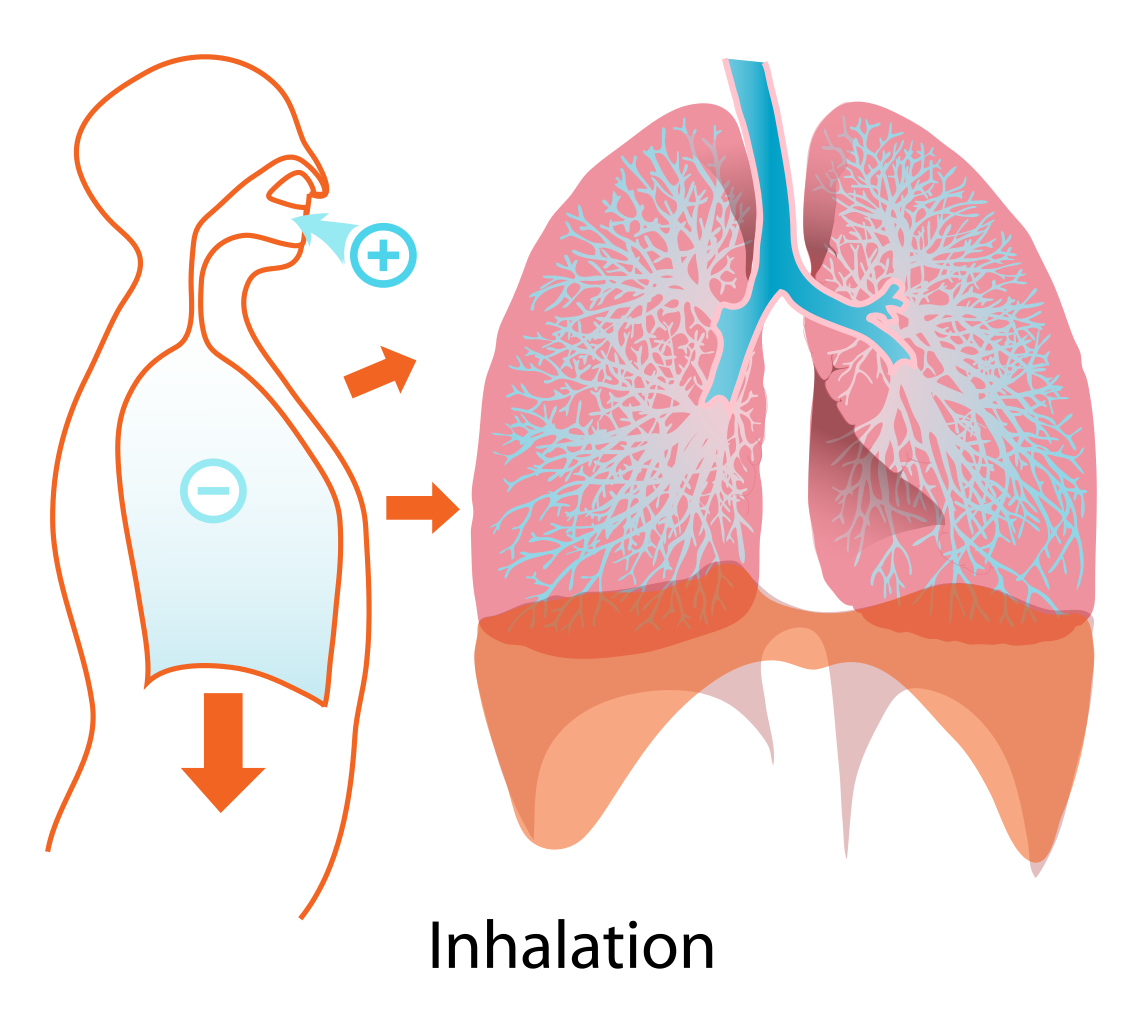
\includegraphics[width=0.9\textwidth]{images/inhalation.png}
\end{minipage}%
\begin{minipage}{.5\textwidth}
\centering
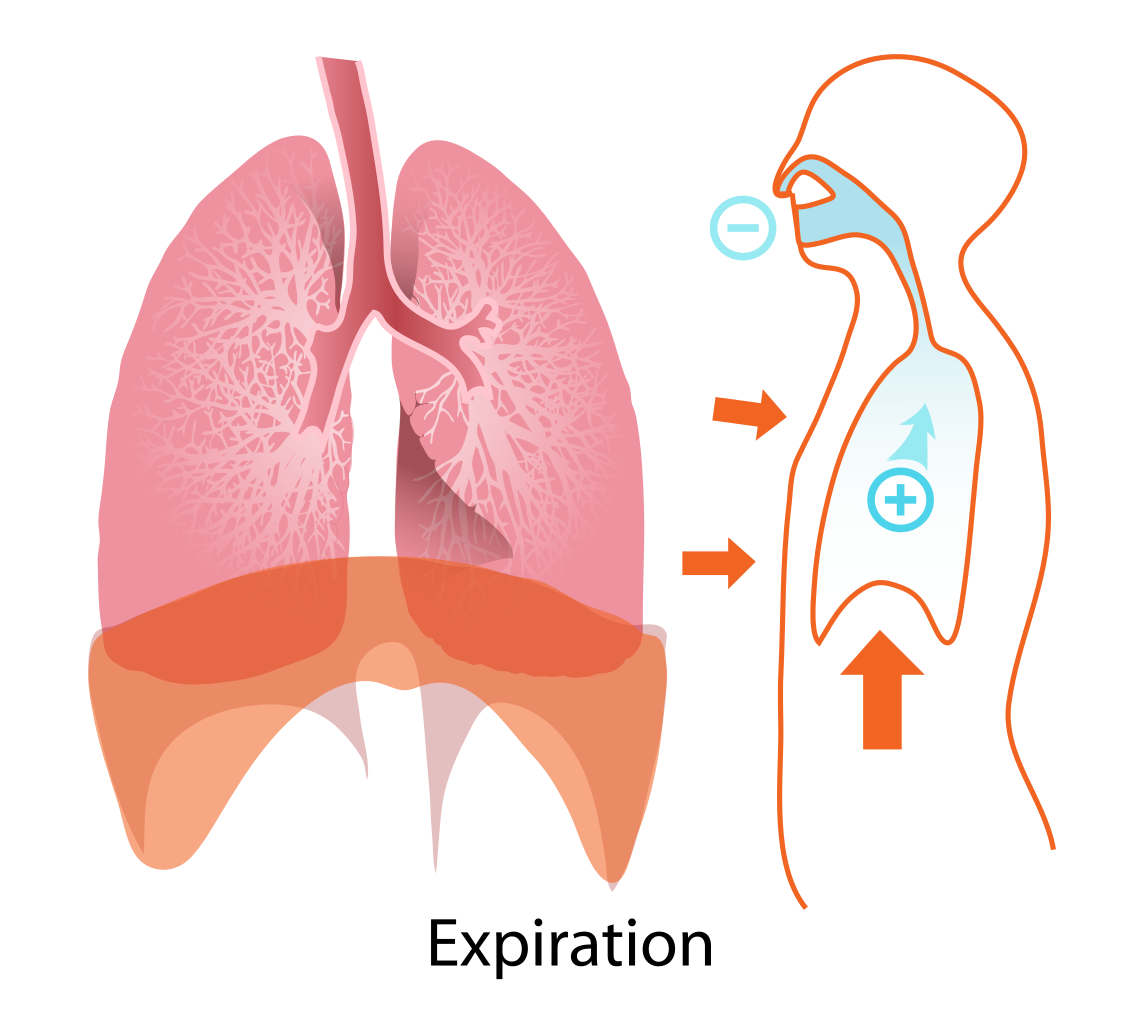
\includegraphics[width=0.9\textwidth]{images/exhalation.png}
\end{minipage}
\caption{La gradiente de presión ($P_{alv}-P_{atm}$) determina el
  flujo de aire dentro y fuera de los pulmones. Las presiones
  mostradas son relativas. Durante la inspiración, la presión
  intrapulmonar cae por debajo de la atmosférica (signo negativo
  frente a signo positivo). Durante la exhalación, la presión
  intrapulmonar se eleva por encima de la atmosférica (signos
  invertidos). Crédito de la imagen: LadyofHats (Mariana Ruiz
  Villarreal) vía Wikimedia Commons, dominio público.}
\label{fig:pressures}
\end{figure}

\subsection*{Medición de los cambios en el volumen de aire durante la respiración - espirometría}

Podemos medir el volumen de aire inhalado o exhalado durante la
respiración con el uso de un espirómetro. Hay varios tipos diferentes
de espirómetro (para revisión ver \cite{schlegelmilch2011pulmonary}).

El tipo que utilizaremos en esta práctica tiene un \emck{built-in
  pressure transducer}. El sujeto respira en un tubo y el aire después
pasa por un filtro, los cuales ayudan a asegurar que el flujo de aire
sea laminar. En el centro del dispositivo hay una pantalla de malla
delgada llamado \emck{pneumotach} que actúa como un resistor. Bajo
condiciones de flujo laminar, la caída de presión a través de una
resistencia es proporcional a la velocidad de flujo de un fluido (gas
o líquido), según lo descrito por la Ley de Poiseuille:

\begin{equation}
Q=\frac{\Delta P \pi r^{4}}{8 l \eta}
\label{eq:presion}
\end{equation},

donde $Q$ es la velocidad de flujo, $\Delta P$ es la diferencia de
presión entre dos puntos, $\eta$ es la viscosidad del fluido, y $r$ y
$l$ son el radio y la longitud del tubo a través del cual el flujo
ocurre.

Por lo tanto, a medida que el sujeto respira y el aire se mueve a
través de la malla, hay una caída de presión que es proporcional a la
velocidad del flujo de aire. Tubos en los dos lados de la malla
transmiten estas presiones a un transductor, que toma la diferencia de
presión entre los dos puntos (P1-P2), dándonos la velocidad de
flujo. Nota que la diferencia de presión será positivo o negativo
dependiendo de si el sujeto está exhalando o inhalando,
respectivamente. Integrar la velocidad de flujo en el tiempo entonces
nos da el volumen de aire exhalado o inhalado.

\begin{figure}[h!]
\centering
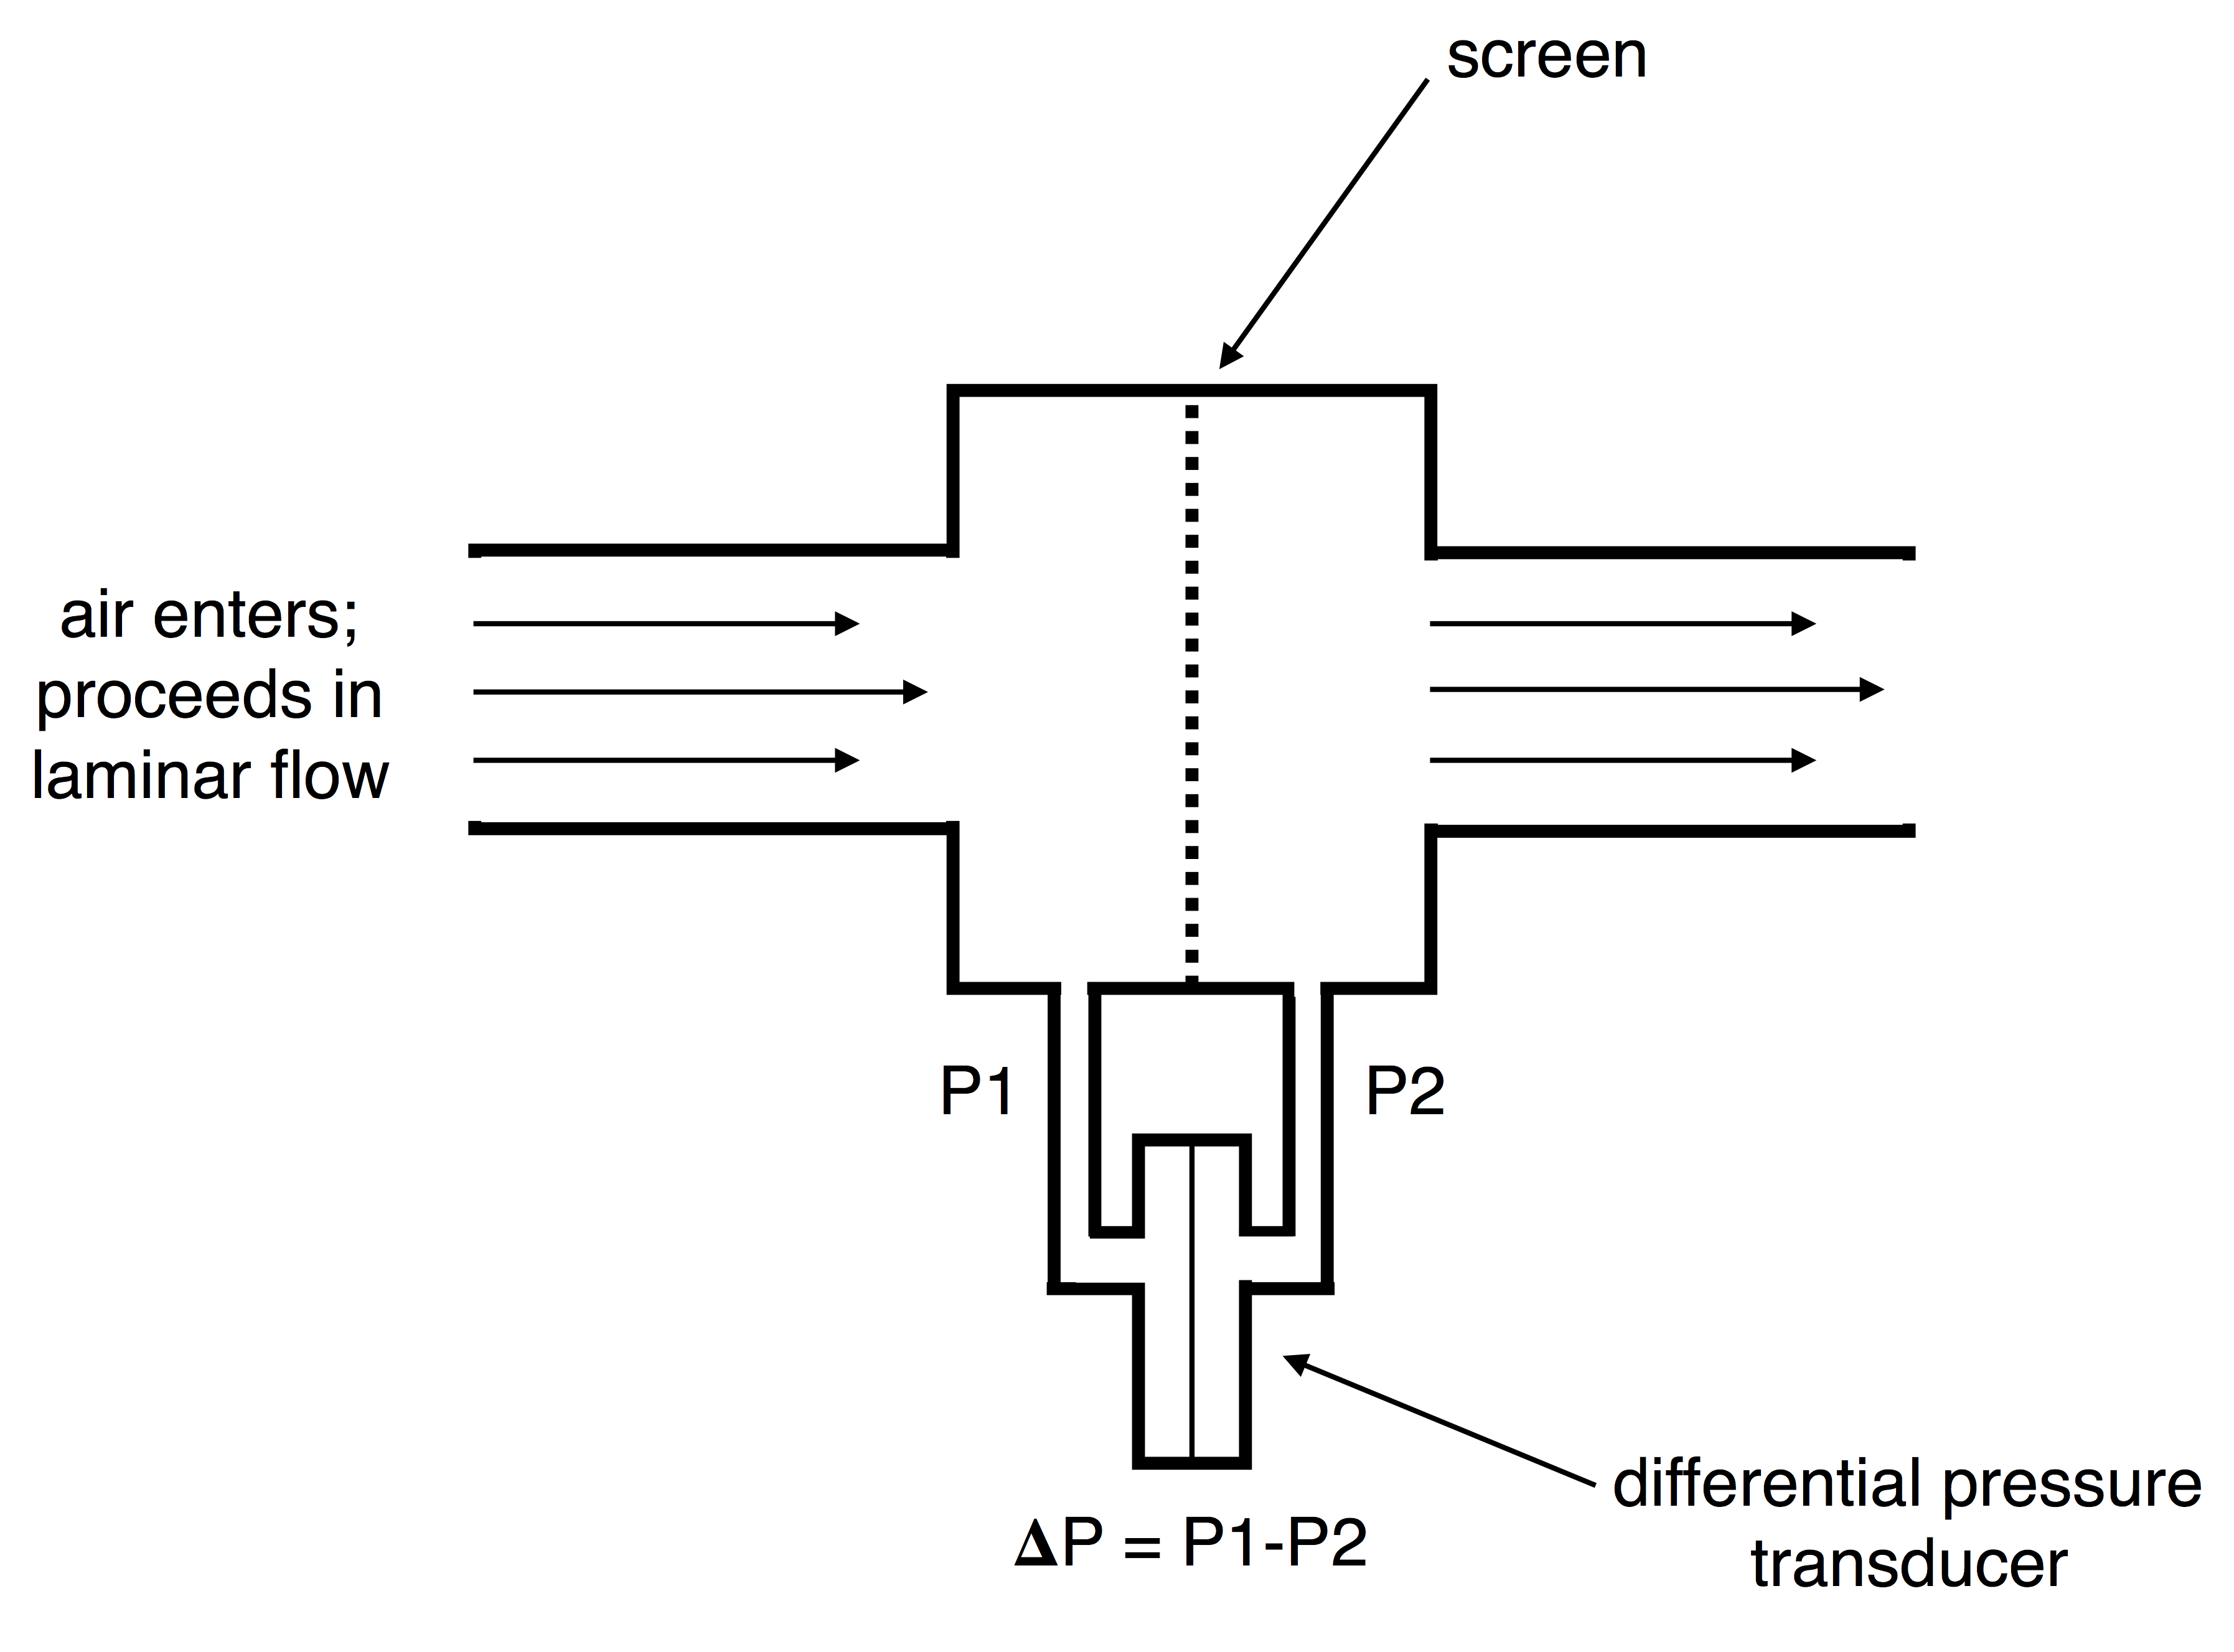
\includegraphics[width=0.7\textwidth]{images/pneumotach.png}
\caption{Esquema de un espirómetro que utiliza un transductor de
  presión diferencial. Credito de imagen: Erin C. McKiernan, CC BY.}
\label{fig:pneumotach}
\end{figure}

\subsection*{Volúmenes y capacidades pulmonares}

Al analizar el espirograma podemos estimar diferentes volúmenes y
capacidade pulmonares (Fig. \ref{fig:volsCaps})
\cite{guyton20006textbook,openStax2016resp}. Los 3 volúmenes y 2
capacidades que se pueden medir con espirometría son:

\begin{itemize}
\item \textbf{\emck{volumen tidal (TV)}}: volumen de aire inhalado y
  exhalado en condiciones normales de reposo
\item \textbf{volumen de reserva inspiratoria \emck{inspiratory
    reserve volume (IRV)}}: volumen adicional de aire que puede ser
  inhalado más allá del volumen tidal cuando se realiza una fuerza
  inspiratoria máxima
\item \textbf{volumen de reserva expiratoria (ERV)}: volumen adicional
  de aire que se puede ser exhalado más allá del volumen tidal cuando
  se realiza una fuerza expiratoria máxima
\item \textbf{capacidad inspiratoria (IC)}: la suma de IRV y TV, es
  decir la cantidad total de aire que una persona puede inhalar
\item \textbf{capacidad vital (VC)}: la suma de IRV, TV y ERV; o, la
  suma de IC y ERV, es decir, el volumen máximo de aire que puede ser
  exhalado con fuerza e inhalando con la fuerza máxima
\end{itemize}

El volumen de aire restante en los pulmones después de la exhalación
máxima, llamado el volumen residual, no se puede medir con
espirometría \cite{guyton20006textbook}. Debido a la contribución de
este volumen a la capacidad residual funcional (FRC) y la capacidad
pulmonar total (TLC), estas capacidades tampoco son medibles con esta
tecnica.

Los volúmenes y capacidades medibles pueden variar hasta un 25\% entre
hombres y mujeres \cite{guyton20006textbook}. Estos valores también varían
con la edad, el estado atlético y ciertas enfermedades respiratorias.

\begin{figure}[h!]
\centering
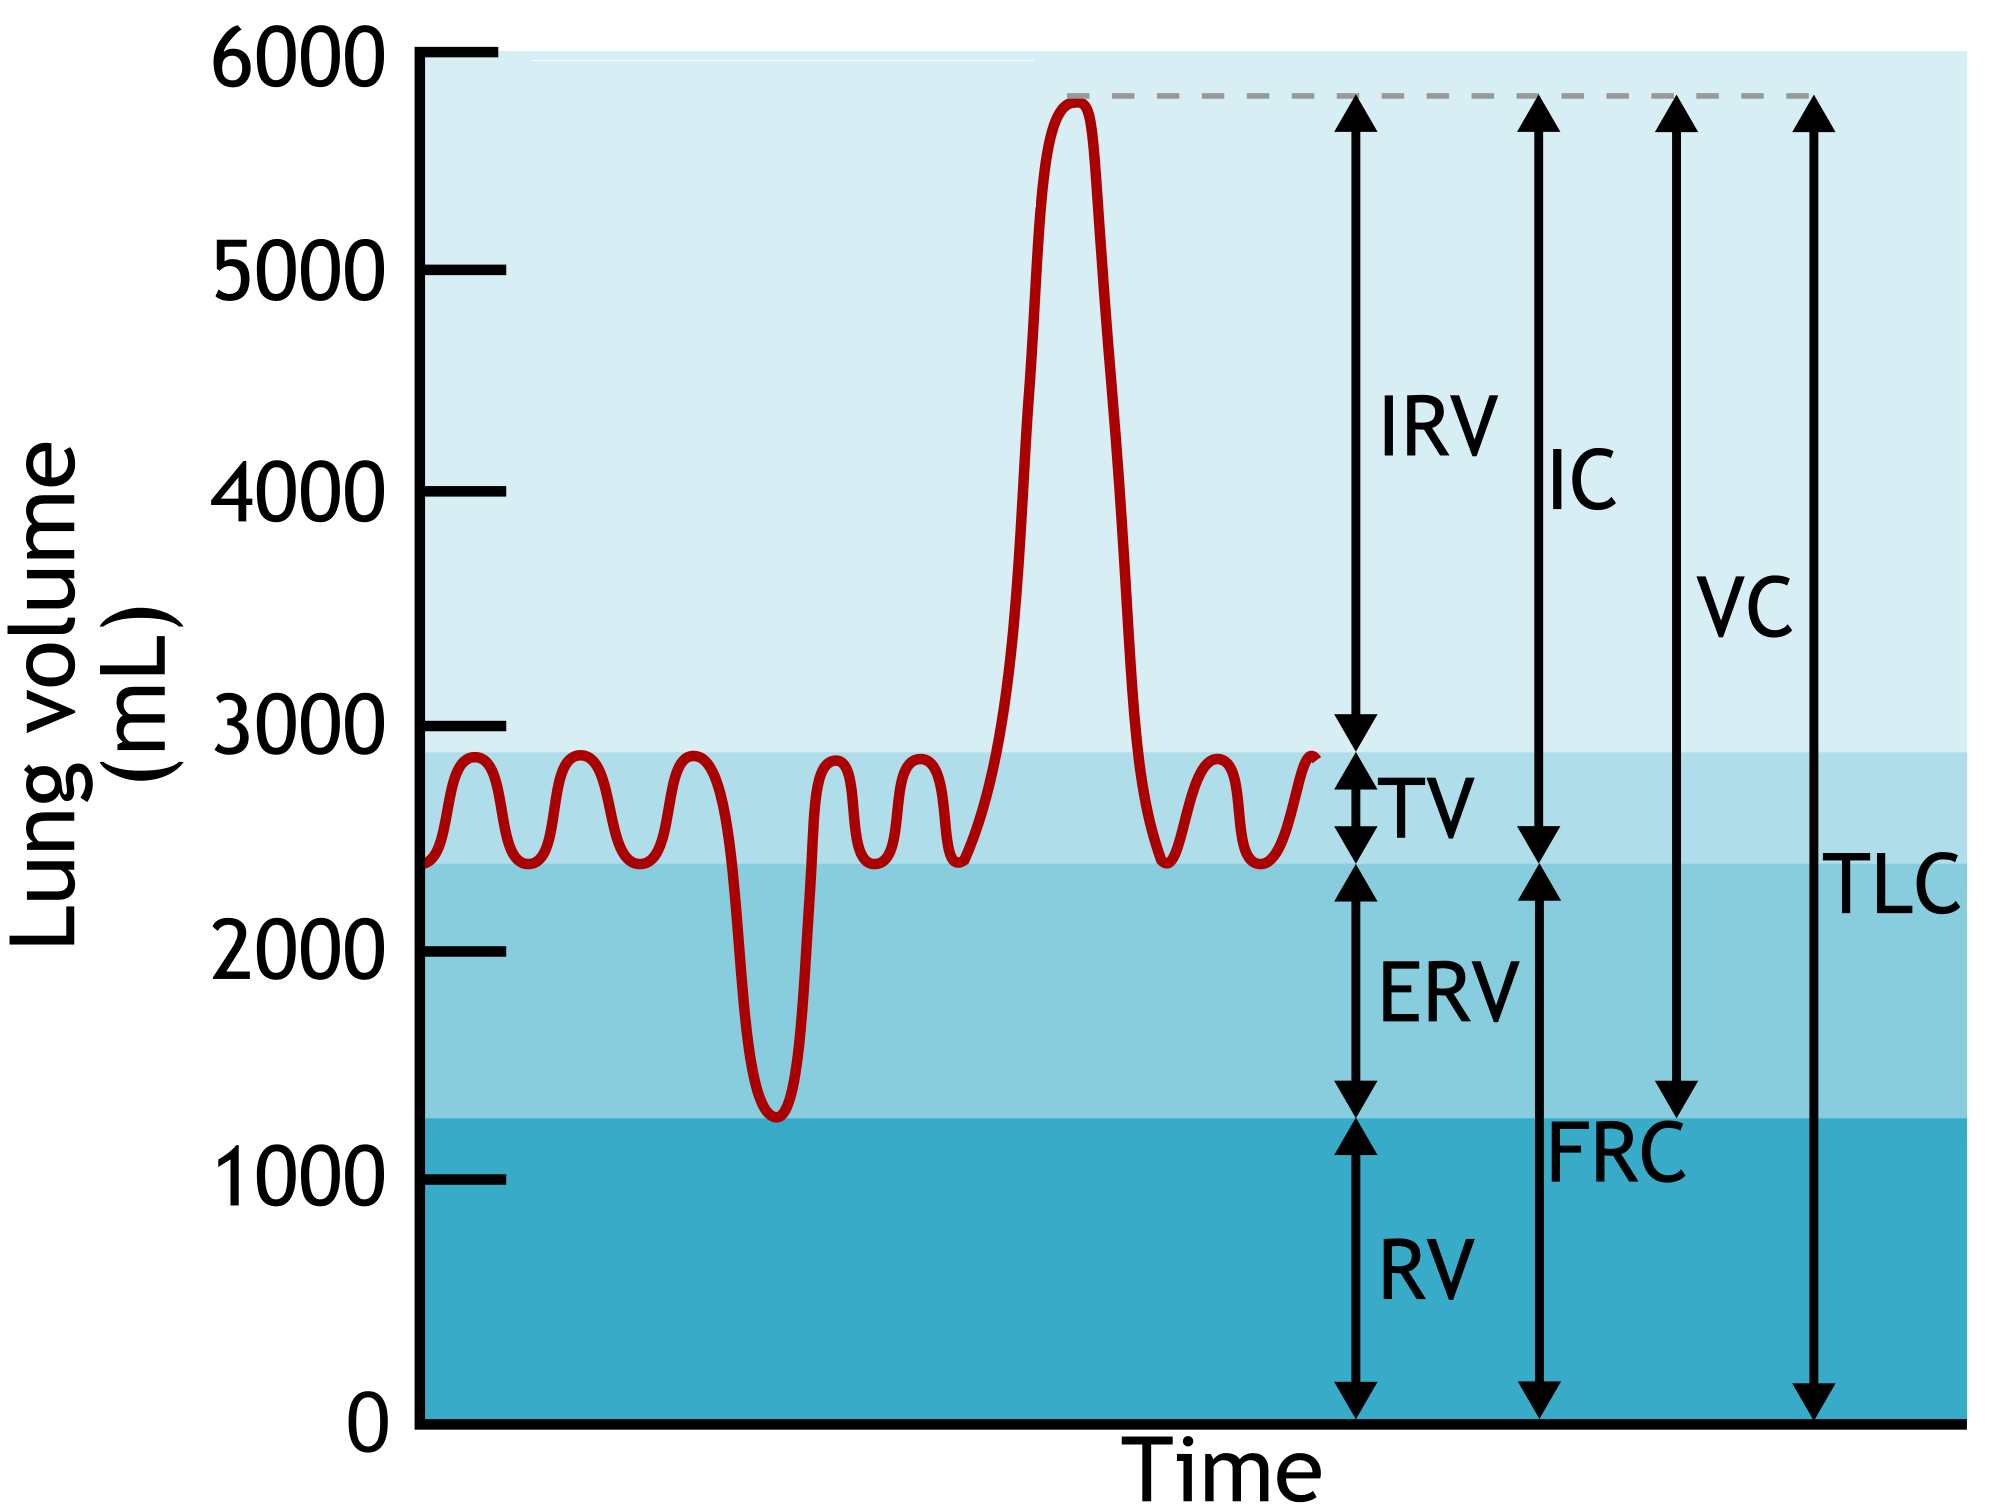
\includegraphics[width=0.8\textwidth]{images/volumesCapacities.png}
\caption{Volúmenes y capacidades inspiratorias. El sujeto toma dos
  respiraciones normales dentro y fuera, seguido por \emck{followed
    by?} de una inspiración normal y luego una expiración máxima,
  luego dos respiraciones normales de nuevo, seguidas de un máximo
  insp.  Crédito de imagen: Michal Komorniczak via Wikimedia Commons,
  CC BY-SA.}
\label{fig:volsCaps}
\end{figure}

\section*{PROCEDIMIENTO}

Antes de comenzar, asegúrese de tener todo el equipo necesario y
ha instalado el software de grabación en su computadora o
teléfono inteligente. Los siguientes pasos lo guiarán en el montaje del
equipo y realización los registros \emck{recordings?}.

\subsection*{1. Montar el espirómetro}

Si su espirómetro está recién comprado, tendrá que realizar todo los
siguientes pasos para armar el dispositivo. Si has usado el
dispositivo anteriormente, solo los pasos ? y ? son necesarios.

\vspace{0.2cm}

\begin{enumerate}
\item Presione los dos pestillos \emck{latches?} en la parte superior
  del mango \emck{handle?} para que se mueven hacia afuera
\item Inserte la cabeza de flujo en el mango y presione los pestillos
  \emck{in to lock in place}
\item Coloque el filtro bacteriano en el lado de la cabeza de flujo
  marcado `inlet'
\item Coloque la boquilla desechable en el extremo del filtro
\end{enumerate}

\vspace{0.2cm}

Cuando su espirómetro está ensamblado \emck {assembled} correctamente,
debería verse así:

\vspace{0.2cm}

\begin{figure}[h!]
\begin{center}
\begin{minipage}{.5\textwidth}
\centering
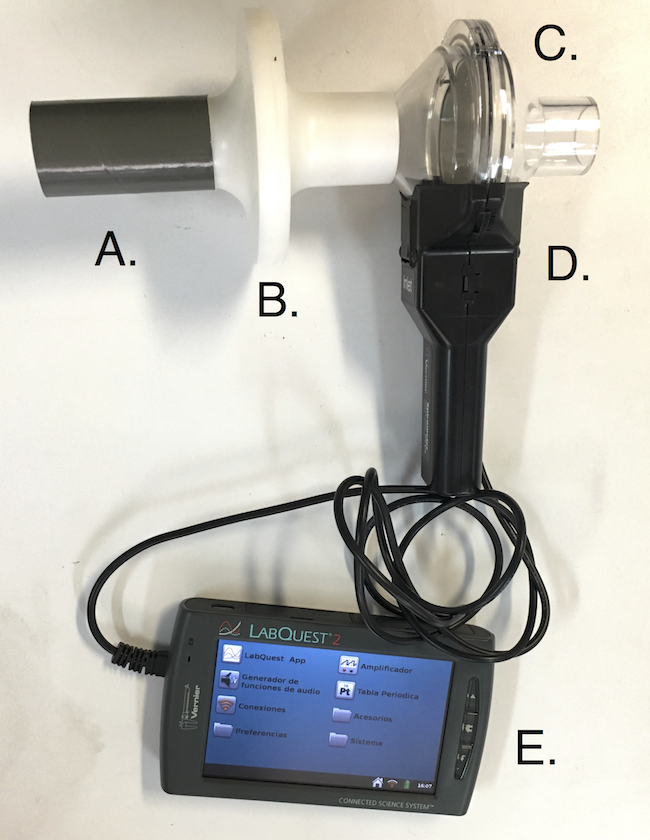
\includegraphics[width=0.9\textwidth]{images/spirometer.png}
\end{minipage}%
\begin{minipage}{.43\textwidth}
\centering
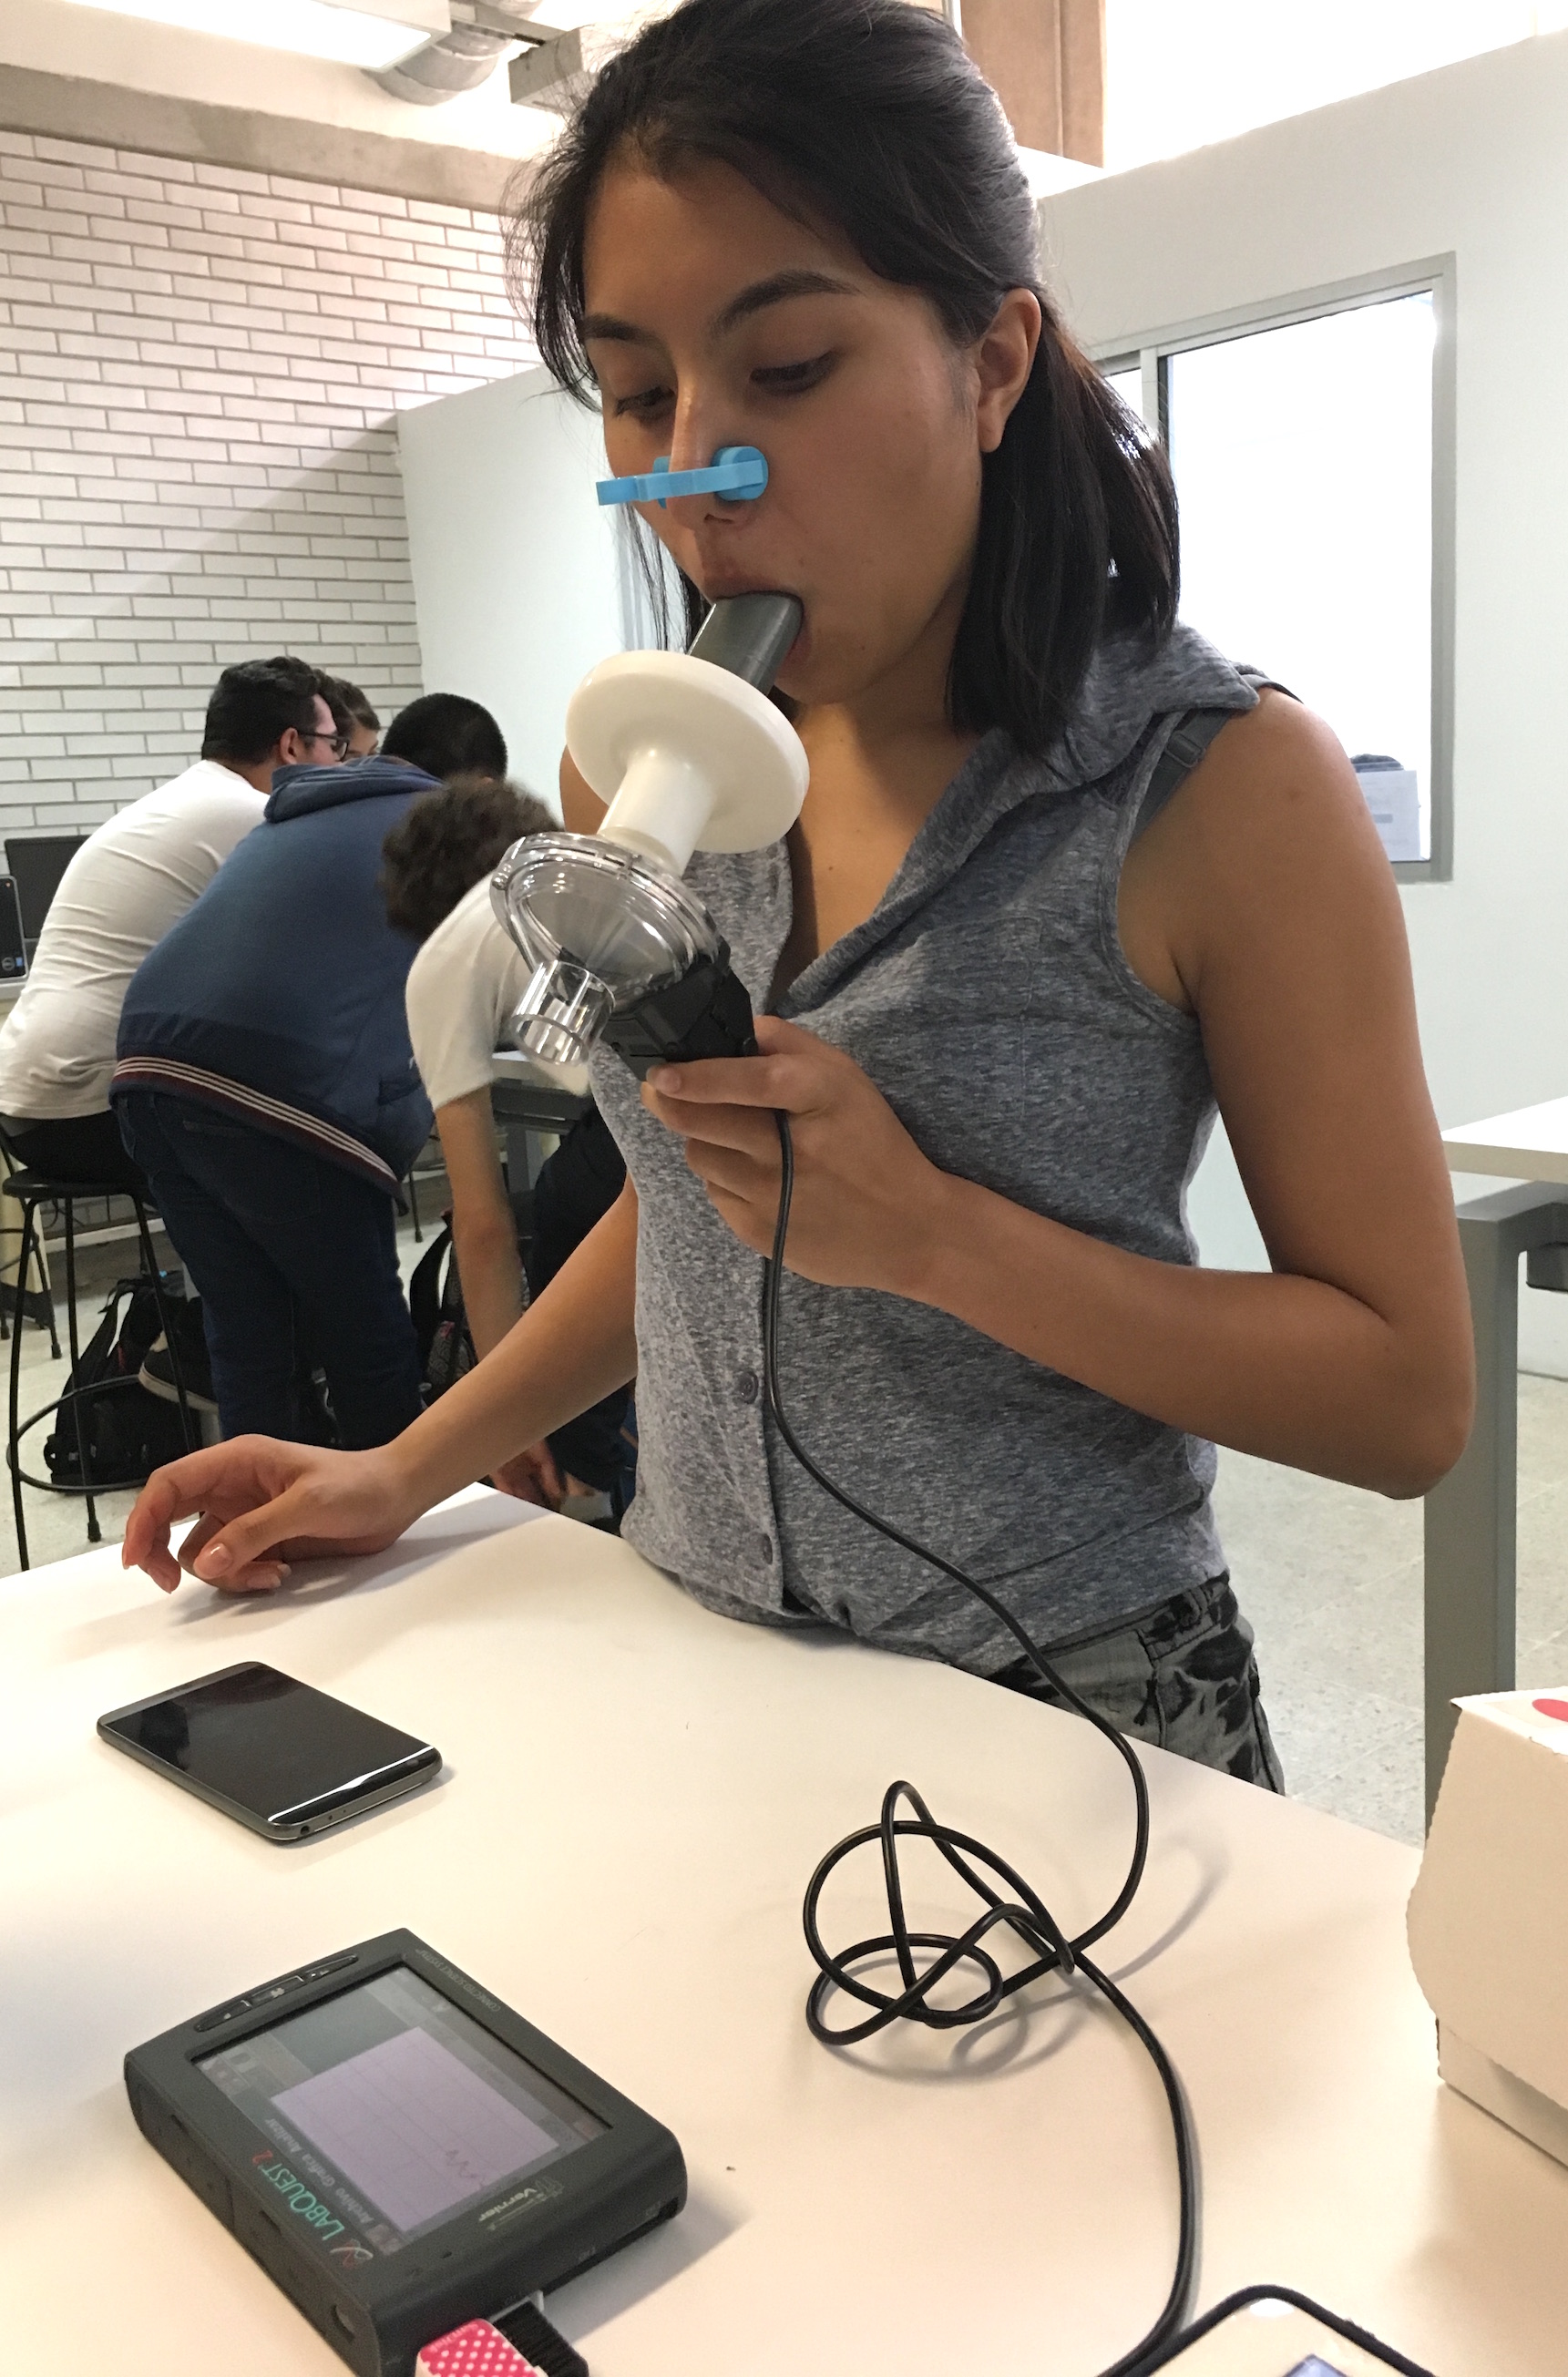
\includegraphics[width=0.9\textwidth]{images/spiro_breathing.JPG}
\end{minipage}
\end{center}
\caption{Izquierda: Espirómetro completamente ensamblado, que muestra
  el tubo de respiración desechable (A.), filtro bacteriano (B.),
  revestimiento \emck{encasing?} de plástico que contiene la malla (C.),
  revestimiento de plástico que contiene transductor de
  presión diferencial (D.) e interfaz LabQuest (E.). Derecha: Estudiante 
  usando un espirómetro durante la práctica. Credito de imagen: ?, CC BY}
\label{fig:spirAssembly}
\end{figure}

\subsection*{2. Pruebe el espirómetro}

\begin{enumerate}
\item Conecte el espirómetro a la interfaz (computadora o dispositivo
  portátil LabQuest 2)
\item Abra el software LabQuest y explore las diferentes funciones
\item Dígale al sujeto que inhale y exhale en la boquilla del espirómetro
\item Verifique que la interfaz muestre los cambios correspondientes
en volumen mientras que el sujeto respira
\item Intente guardar y exportar un archivo de datos (use el formato txt)
\end{enumerate}

\subsection*{3. Configurar grabaciones EMG}

El Muscle SpikerBo de Backyard Brains viene completamente ensamblado y
listo para registrar. Solo tiene que conectar la pila, los cables y
electrodos.

\vspace{0.2cm}

\begin{enumerate}
\item Conecte la batería de 9V a sus terminales en el Muscle SpikerBox
\item Conecte el cable negro/azul o verde al puerto (\emck{port?})
  correspondiente de computadora o teléfono inteligente en el Muscle
  SpikerBox; tenga en cuenta que el cable del teléfono inteligente es
  direccional, asegúrese de tener el lado correcto insertado en el
  dispositivo
\item Conecte el otro lado del cable negro/azul o verde a su
  computadora o teléfono inteligente
\item Conecte el cable naranja a su puerto correspondiente en el Muscle
SpikerBox
\item Coloque los electrodos de superficie sobre el músculo de interés
  aproximadamente ? cm separados y orientados en paralelo a las
  fibras musculares
\item Conecte cada una de las pinzas rojas de cocodrilo en los
  terminales del cable naranja a uno de los electrodos de superficie;
  asegúrese de que los clips metálicos no se toquen y trate de evitar
  enredar los cables
\item agarra el clip negro de cocodrilo (referencia) en su mano, o
  conéctelo a otro electrodo de superficie en el dorso de su mano o en
  otra área lejos del sitio de registro

\vspace{0.2cm}

\begin{figure}[h!]
\begin{center}
\begin{minipage}{.55\textwidth}
\centering
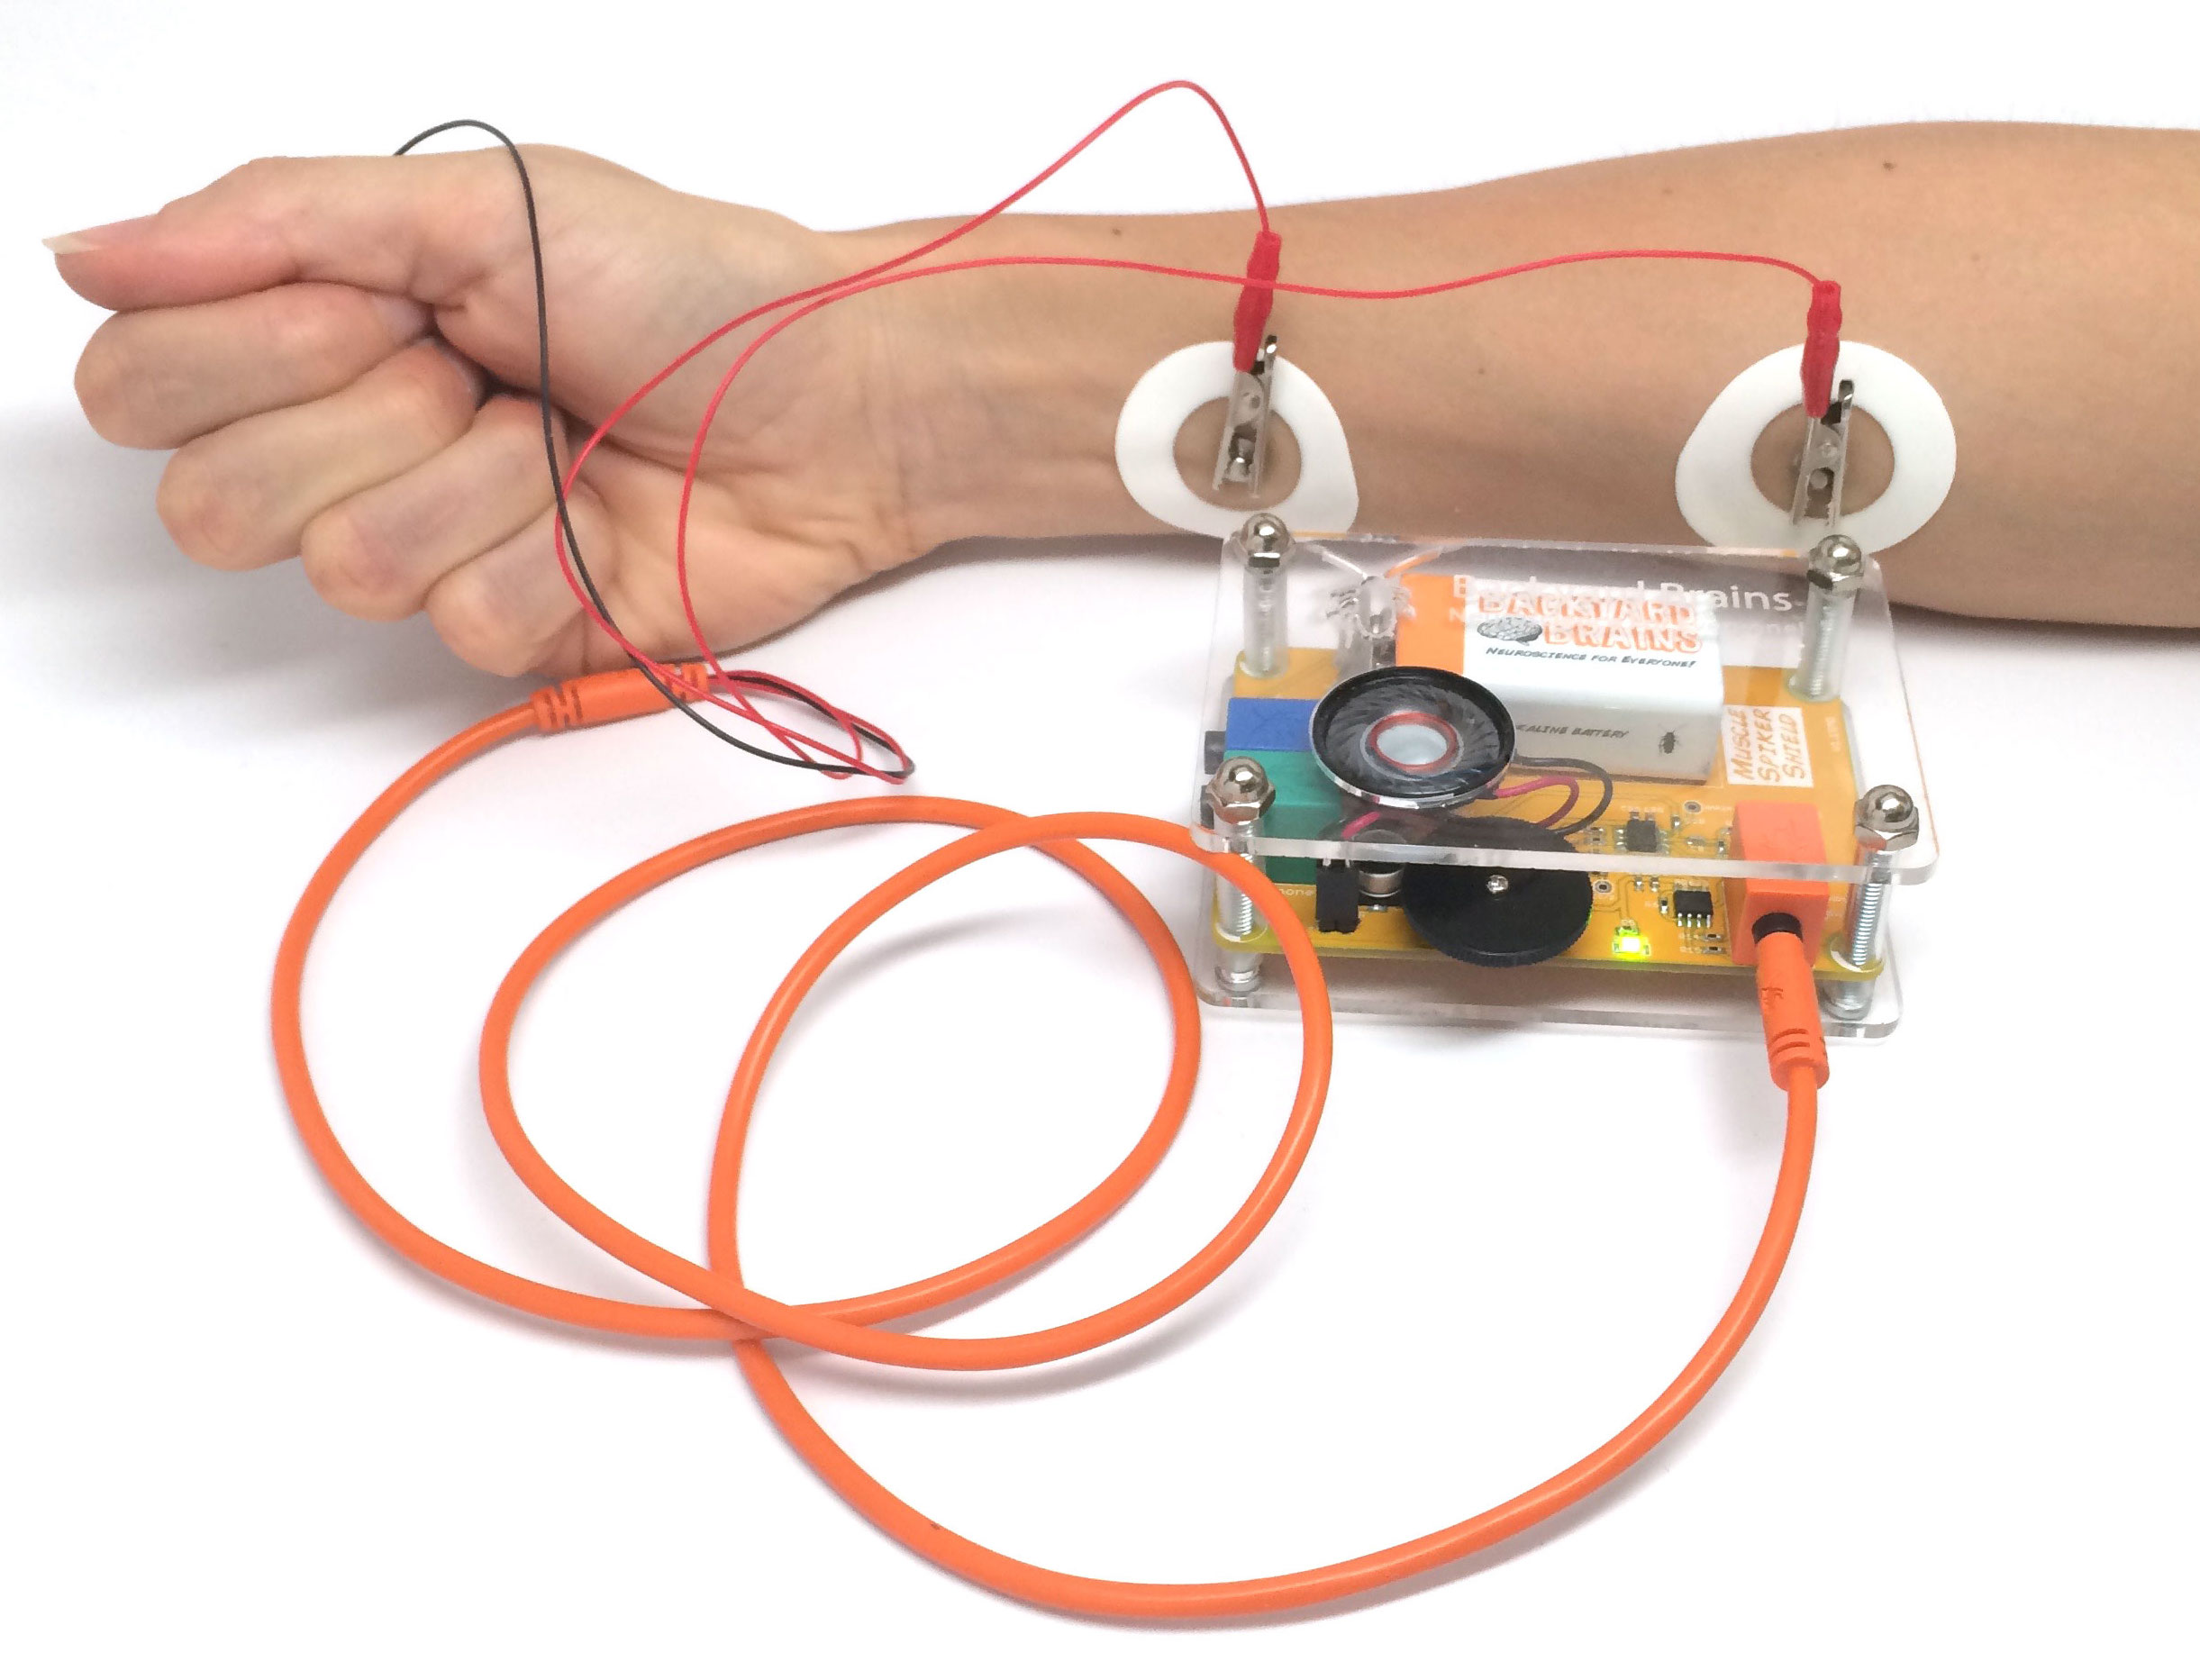
\includegraphics[width=0.9\textwidth]{images/muscleSpikerBox.jpg}
\end{minipage}%
\begin{minipage}{.4\textwidth}
\centering
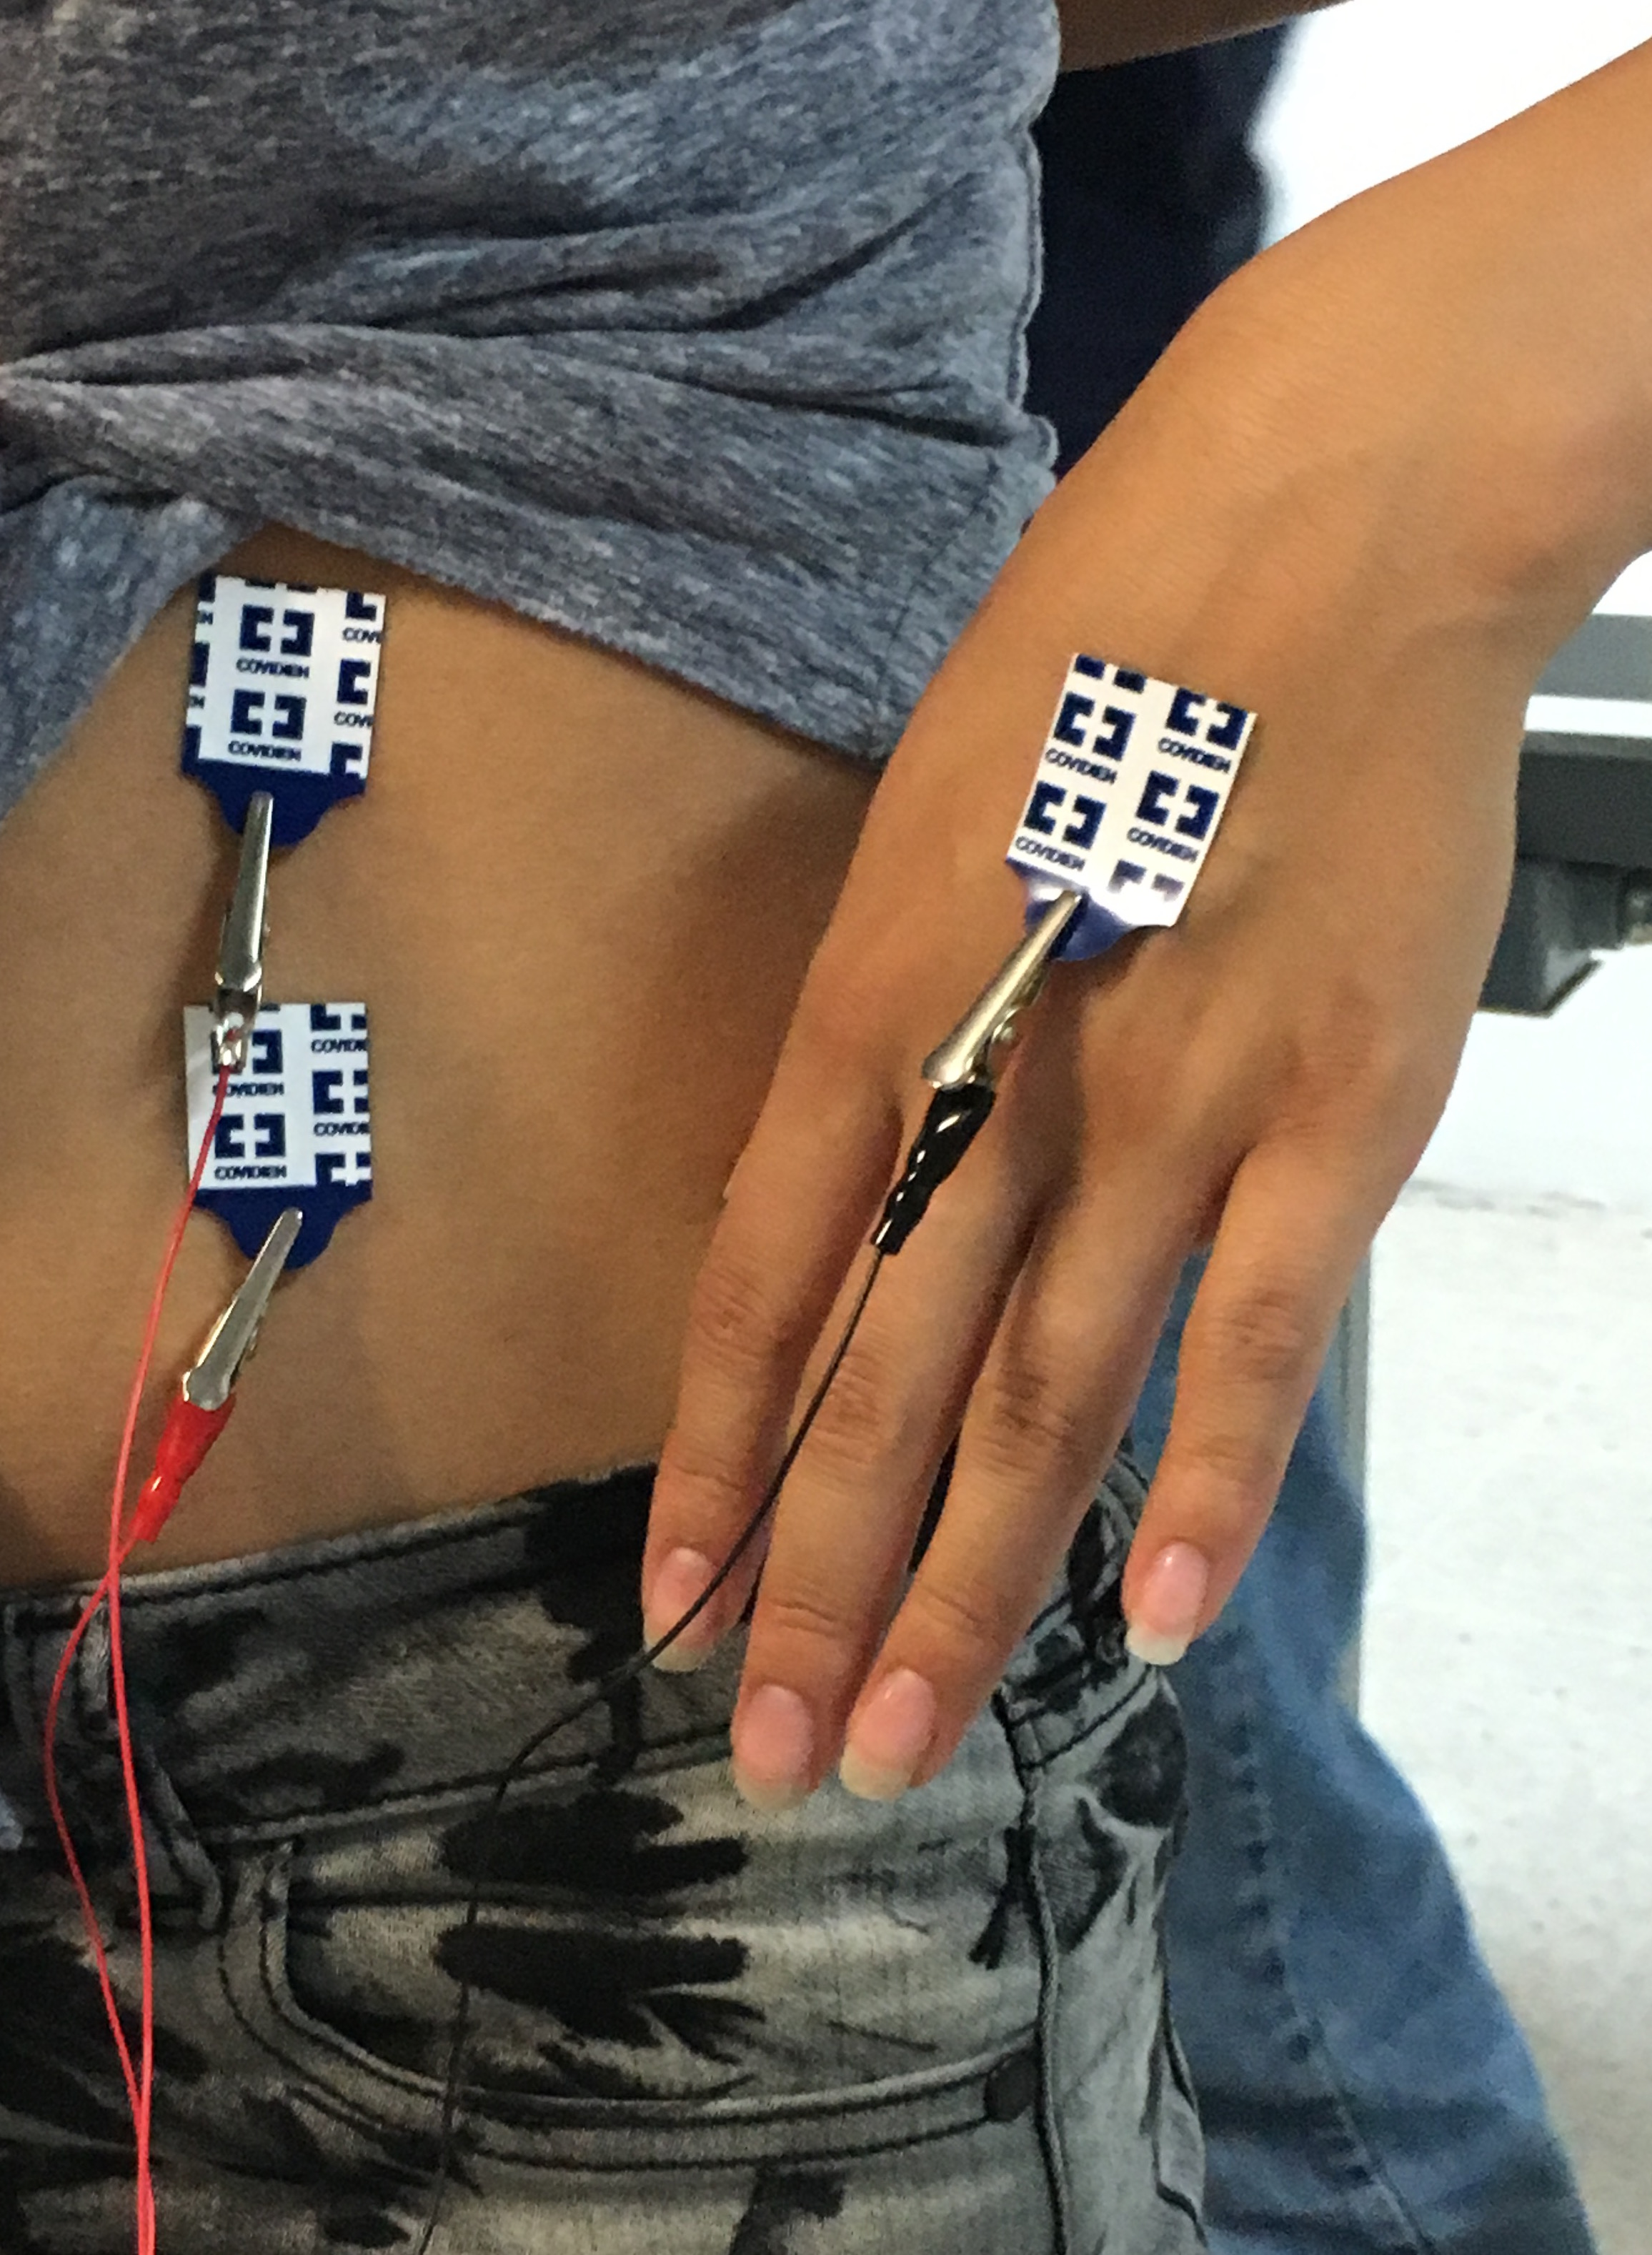
\includegraphics[width=0.8\textwidth]{images/electrodeAb.JPG}
\end{minipage}
\end{center}
\caption{\textit{Izquierda}: Configuración de EMG con electrodos
  conectados al Muscle SpikerBox. (No se muestra la conexión a la
  computadora o teléfono inteligente). Crédito del imagen: Backyard
  Brains, CC BY SA. \textit{Derecha}: Electrodos de superficie
  colocados para registrar del músculo recto¡us abdominus durante
  expiración (\emck{mejor exhalación?}) forzada. Crédito del
  imagen: ?, CC BY}
\label{fig:spirAssembly}
\end{figure}

\item Para mejorar la señal EMG, el área donde los electrodos serán
  colocados puede limpiarse con alcohol antes de la colocación;
  esperar hasta el área está seca para colocar los electrodos
\item El gel de electrodos se puede colocar para mejorar la
  conducción, pero muchas veces no es necesario
\item Para evitar artefactos de ruido, asegúrese de que ninguna ropa
  toque los electrodos o cepillar contra \emck{no clothing is touching
    the electrodes or brushing against} los cables durante el registro
\end{enumerate}
 
\subsection*{4. Prueba los registros EMG}

\begin{enumerate}
\item Encienda el Muscle SpikerBox girando el \emck{black wheel
  switch} en el lado, una luz verde debe encenderse; tenga en cuenta
  que los electrodos deben estar conectados antes de encender el
  dispositivo y desconectados solo después de que el dispositivo
  esté apagado para evitar un ruido desagradable!
\item Abra el software de registro de Backyard Brains y explore los
  controles y las configuraciones (para obtener más información sobre
  el uso del software, consulte \cite{spikeRecorder})

\begin{figure}[h!]
\centering
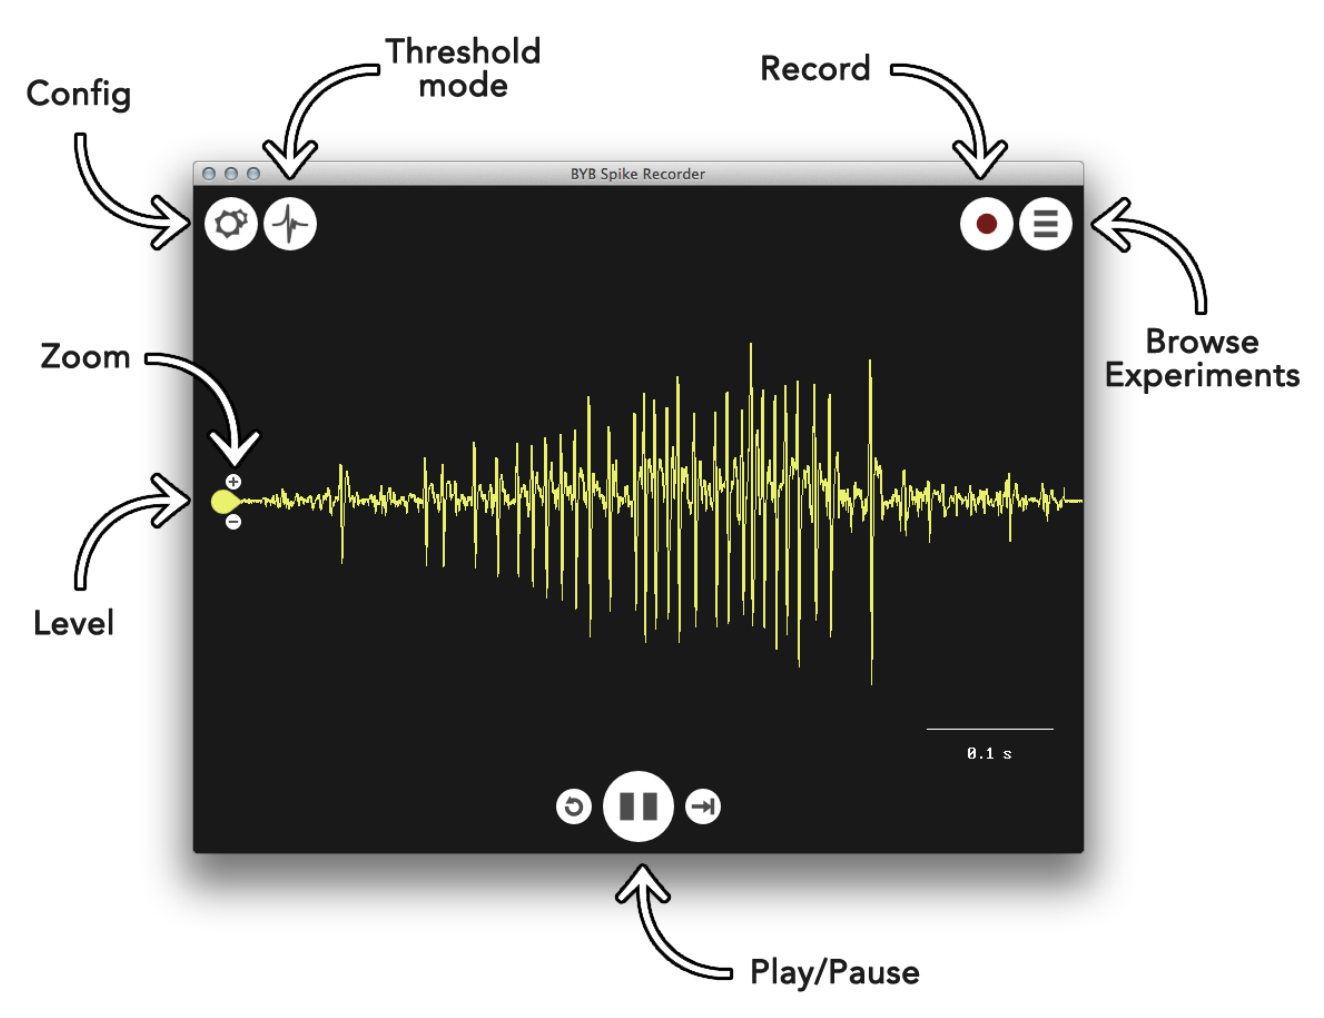
\includegraphics[width=0.8\textwidth]{images/BBrecorder.png}
\caption{Interfaz de software de registro. Crédito de imagen: Backyard
  Brains, CC BY SA.}
\label{fig:recorder}
\end{figure}

\item Coloque \emck{smap} sus dedos cerca del dispositivo de registro;
  si ves un artefacto correspondiente en la pantalla, esto significa
  que estás grabando solo audio; para comenzar a registrar la
  actividad muscular, ajuste la configuración presionando el botón
  `Config ' (Fig. \ref{fig:recorder}) (ver
  \cite{spikeRecorder} para más detalles)
\item Pídale al sujeto que brevemente contraiga y relaje el músculo de
  interés
\item Verifique que se observen potenciales eléctricos durante la
  contracción; verifica tu relación señal/ruido; si la señal es
  demasiado pequeña, puede ajustar la ganancia \emck{gain} girando el
  interruptor de la \emck{wheel switch} hacia la derecha
\item Try saving a recording to your computer or smartphone (format
  will be .wav)
\end{enumerate}

\subsection*{5. Recoge tus datos}

\begin{enumerate}
\item Asegúrese de que el EMG esté listo para registrar, y el sujeto
  tenga el espirómetro en la mano
\item Coloque el clip azul sobre la nariz del sujeto; si encuentran
  que es incómodo, simplemente pídales que se sujeten la nariz
  \emck{hold their nose} durante el ejercicio
\item Indique al sujeto que cuando comience el registrp, 
realizarán la siguiente secuencia:
\begin{itemize}
\item dos respiraciones normales
\item una inhalación normal seguida de una exhalación forzada máxima
\item dos respiraciones normales
\item inhalación máxima forzada seguida de una exhalación normal
\item dos respiraciones normales
\item inhalación máxima forzada seguida de una exhalación máxima forzada
\item dos respiraciones normales
\end{itemize}
\item Puedes poner una imagen como la que se ve en la
  Fig. \ref{fig:volsCaps} frente al sujeto e instruirlos
  verbalmente para ayudarlos recordar la secuencia
\item Como está grabando en dos dispositivos diferentes, debe hacer lo
  mejor para sincronizar manualmente los registros; tener una persona
  en cargo de presionar registrar en el EMG y otro a cargo del
  registro de espirómetro
\item Cuente hasta 3 y haga que las dos personas presionen `grabar' en
  los diferentes dispositivos al mismo tiempo
\item Al final de la secuencia, cuente hasta 3 nuevamente y haga que las
  dos personas terminan las grabaciones al mismo tiempo
\item Guarde los datos en su computadora o teléfono inteligente; si
  trabaja en el LabQuest2, puede guardar los datos en una memoria
  USB
\item Los EMG deben guardarse y exportarse en .wav y los espirogramas en
  formato .txt para el análisis
\item Si esta coleccionando datos de sujetos adicionales, limpie el
  espirómetro con toallitas de alcohol y reemplazar la boquilla
  desechable con una nueva antes de proceder
\end{enumerate}

\section*{ACKNOWLEDGMENTS}
Este trabajo fue apoyado por l aDirección General de Asuntos del
Personal Académico, Programa de Apoyo a Proyectos para la Innovación y
Mejoramiento de la Enseñanza en la Universidad Nacional Autónoma de
México (UNAM-DGAPA-PAPIME clave PE213817).
 
% BIBLIOGRAPHY
\begin{small}
\bibliography{resp}
\end{small}

\end{document}
